\documentclass{article}

\usepackage[utf8]{inputenc}
\usepackage{fullpage}
\usepackage{amsmath, amssymb, amsfonts, amsthm}
\usepackage{mathtools}
\usepackage{twoopt}
\usepackage{graphicx, subfig, float}
\usepackage{listings, xcolor}
\usepackage{placeins}
\usepackage{babel}
\usepackage{verbatim}

\usepackage{multicol}
\setlength{\columnsep}{0cm}

\parindent 0pt

% special letters:

\newcommand{\N}{\mathbb{N}}
\newcommand{\Z}{\mathbb{Z}}
\newcommand{\Q}{\mathbb{Q}}
\newcommand{\R}{\mathbb{R}}
\newcommand{\C}{\mathbb{C}}
\newcommand{\K}{\mathbb{K}}
\newcommand{\T}{\mathbb{T}}
\newcommand{\E}{\mathbb{E}}
\newcommand{\V}{\mathbb{V}}
\renewcommand{\S}{\mathbb{S}}
\renewcommand{\P}{\mathbb{P}}
\newcommand{\1}{\mathbbm{1}}

% quantors:

\newcommand{\Forall}{\forall \,}
\newcommand{\Exists}{\exists \,}
\newcommand{\ExistsOnlyOne}{\exists! \,}
\newcommand{\nExists}{\nexists \,}
\newcommand{\ForAlmostAll}{\forall^\infty \,}

% MISC symbols:

\newcommand{\landau}{{\scriptstyle \mathcal{O}}}
\newcommand{\Landau}{\mathcal{O}}


\newcommand{\eps}{\mathrm{eps}}

% graphics in a box:

\newcommandtwoopt
{\includegraphicsboxed}[3][][]
{
  \begin{figure}[!h]
    \begin{boxedin}
      \ifthenelse{\isempty{#1}}
      {
        \begin{center}
          \includegraphics[width = 0.75 \textwidth]{#3}
          \label{fig:#2}
        \end{center}
      }{
        \begin{center}
          \includegraphics[width = 0.75 \textwidth]{#3}
          \caption{#1}
          \label{fig:#2}
        \end{center}
      }
    \end{boxedin}
  \end{figure}
}

% braces:

\newcommand{\pbraces}[1]{{\left  ( #1 \right  )}}
\newcommand{\bbraces}[1]{{\left  [ #1 \right  ]}}
\newcommand{\Bbraces}[1]{{\left \{ #1 \right \}}}
\newcommand{\vbraces}[1]{{\left  | #1 \right  |}}
\newcommand{\Vbraces}[1]{{\left \| #1 \right \|}}
\newcommand{\abraces}[1]{{\left \langle #1 \right \rangle}}
\newcommand{\round}[1]{\bbraces{#1}}

\newcommand
{\floorbraces}[1]
{{\left \lfloor #1 \right \rfloor}}

\newcommand
{\ceilbraces} [1]
{{\left \lceil  #1 \right \rceil }}

% special functions:

\newcommand{\norm}  [2][]{\Vbraces{#2}_{#1}}
\newcommand{\diam}  [2][]{\mathrm{diam}_{#1} \: #2}
\newcommand{\diag}  [1]{\mathrm{diag} \: #1}
\newcommand{\dist}  [1]{\mathrm{dist} \: #1}
\newcommand{\mean}  [1]{\mathrm{mean} \: #1}
\newcommand{\erf}   [1]{\mathrm{erf} \: #1}
\newcommand{\id}    [1]{\mathrm{id} \: #1}
\newcommand{\sgn}   [1]{\mathrm{sgn} \: #1}
\newcommand{\supp}  [1]{\mathrm{supp} \: #1}
\newcommand{\arsinh}[1]{\mathrm{arsinh} \: #1}
\newcommand{\arcosh}[1]{\mathrm{arcosh} \: #1}
\newcommand{\artanh}[1]{\mathrm{artanh} \: #1}
\newcommand{\card}  [1]{\mathrm{card} \: #1}
\newcommand{\Span}  [1]{\mathrm{span} \: #1}
\newcommand{\Aut}   [1]{\mathrm{Aut} \: #1}
\newcommand{\End}   [1]{\mathrm{End} \: #1}
\newcommand{\ggT}   [1]{\mathrm{ggT} \: #1}
\newcommand{\kgV}   [1]{\mathrm{kgV} \: #1}
\newcommand{\ord}   [1]{\mathrm{ord} \: #1}
\newcommand{\grad}  [1]{\mathrm{grad} \: #1}
\newcommand{\ran}   [1]{\mathrm{ran} \: #1}
\newcommand{\graph} [1]{\mathrm{graph} \: #1}
\newcommand{\Inv}   [1]{\mathrm{Inv} \: #1}
\newcommand{\pv}    [1]{\mathrm{pv} \: #1}
\newcommand{\GL}    [1]{\mathrm{GL} \: #1}
\newcommand{\Mod}{\mathrm{Mod} \:}
\newcommand{\Th}{\mathrm{Th} \:}
\newcommand{\Char}{\mathrm{char}}
\newcommand{\At}{\mathrm{At}}
\newcommand{\Ob}{\mathrm{Ob}}
\newcommand{\Hom}{\mathrm{Hom}}
\newcommand{\orthogonal}[3][]{#2 ~\bot_{#1}~ #3}
\newcommand{\Rang}{\mathrm{Rang}}
\newcommand{\NIL}{\mathrm{NIL}}
\newcommand{\Res}{\mathrm{Res}}
\newcommand{\lxor}{\dot \lor}
\newcommand{\Div}{\mathrm{div} \:}
\newcommand{\meas}{\mathrm{meas} \:}

% fractions:

\newcommand{\Frac}[2]{\frac{1}{#1} \pbraces{#2}}
\newcommand{\nfrac}[2]{\nicefrac{#1}{#2}}

% derivatives & integrals:

\newcommandtwoopt
{\Int}[4][][]
{\int_{#1}^{#2} #3 ~\mathrm{d} #4}

\newcommandtwoopt
{\derivative}[3][][]
{
  \frac
  {\mathrm{d}^{#1} #2}
  {\mathrm{d} #3^{#1}}
}

\newcommandtwoopt
{\pderivative}[3][][]
{
  \frac
  {\partial^{#1} #2}
  {\partial #3^{#1}}
}

\newcommand
{\primeprime}
{{\prime \prime}}

\newcommand
{\primeprimeprime}
{{\prime \prime \prime}}

% Text:

\newcommand{\Quote}[1]{\glqq #1\grqq{}}
\newcommand{\Text}[1]{{\text{#1}}}
\newcommand{\fastueberall}{\text{f.ü.}}
\newcommand{\fastsicher}{\text{f.s.}}

% ---------------------------------------------------------------- %
% https://www.overleaf.com/learn/latex/Code_listing

\definecolor{codegreen} {rgb}{0, 0.6, 0}
\definecolor{codegray}    {rgb}{0.5, 0.5, 0.5}
\definecolor{codepurple}{rgb}{0.58, 0, 0.82}
\definecolor{backcolour}{rgb}{0.95, 0.95, 0.92}

\lstdefinestyle{overleaf}
{
    backgroundcolor = \color{backcolour},
    commentstyle = \color{codegreen},
    keywordstyle = \color{magenta},
    numberstyle = \tiny\color{codegray},
    stringstyle = \color{codepurple},
    basicstyle = \ttfamily \footnotesize,
    breakatwhitespace = false,
    breaklines = true,
    captionpos = b,
    keepspaces = true,
    numbers = left,
    numbersep = 5pt,
    showspaces = false,
    showstringspaces = false,
    showtabs = false,
    tabsize = 2
}

% ---------------------------------------------------------------- %
% https://en.wikibooks.org/wiki/LaTeX/Source_Code_Listings

\lstdefinestyle{customc}
{
    belowcaptionskip = 1 \baselineskip,
    breaklines = true,
    frame = L,
    xleftmargin = \parindent,
    language = C,
    showstringspaces = false,
    basicstyle = \footnotesize \ttfamily,
    keywordstyle = \bfseries \color{green!40!black},
    commentstyle = \itshape \color{purple!40!black},
    identifierstyle = \color{blue},
    stringstyle = \color{orange},
}

\lstdefinestyle{customasm}
{
    belowcaptionskip = 1 \baselineskip,
    frame = L,
    xleftmargin = \parindent,
    language = [x86masm] Assembler,
    basicstyle = \footnotesize\ttfamily,
    commentstyle = \itshape\color{purple!40!black},
}

% ---------------------------------------------------------------- %
% https://tex.stackexchange.com/questions/235731/listings-syntax-for-literate

\definecolor{maroon}        {cmyk}{0, 0.87, 0.68, 0.32}
\definecolor{halfgray}      {gray}{0.55}
\definecolor{ipython_frame} {RGB}{207, 207, 207}
\definecolor{ipython_bg}    {RGB}{247, 247, 247}
\definecolor{ipython_red}   {RGB}{186, 33, 33}
\definecolor{ipython_green} {RGB}{0, 128, 0}
\definecolor{ipython_cyan}  {RGB}{64, 128, 128}
\definecolor{ipython_purple}{RGB}{170, 34, 255}

\lstdefinestyle{stackexchangePython}
{
    breaklines = true,
    %
    extendedchars = true,
    literate =
    {á}{{\' a}} 1 {é}{{\' e}} 1 {í}{{\' i}} 1 {ó}{{\' o}} 1 {ú}{{\' u}} 1
    {Á}{{\' A}} 1 {É}{{\' E}} 1 {Í}{{\' I}} 1 {Ó}{{\' O}} 1 {Ú}{{\' U}} 1
    {à}{{\` a}} 1 {è}{{\` e}} 1 {ì}{{\` i}} 1 {ò}{{\` o}} 1 {ù}{{\` u}} 1
    {À}{{\` A}} 1 {È}{{\' E}} 1 {Ì}{{\` I}} 1 {Ò}{{\` O}} 1 {Ù}{{\` U}} 1
    {ä}{{\" a}} 1 {ë}{{\" e}} 1 {ï}{{\" i}} 1 {ö}{{\" o}} 1 {ü}{{\" u}} 1
    {Ä}{{\" A}} 1 {Ë}{{\" E}} 1 {Ï}{{\" I}} 1 {Ö}{{\" O}} 1 {Ü}{{\" U}} 1
    {â}{{\^ a}} 1 {ê}{{\^ e}} 1 {î}{{\^ i}} 1 {ô}{{\^ o}} 1 {û}{{\^ u}} 1
    {Â}{{\^ A}} 1 {Ê}{{\^ E}} 1 {Î}{{\^ I}} 1 {Ô}{{\^ O}} 1 {Û}{{\^ U}} 1
    {œ}{{\oe}}  1 {Œ}{{\OE}}  1 {æ}{{\ae}}  1 {Æ}{{\AE}}  1 {ß}{{\ss}}  1
    {ç}{{\c c}} 1 {Ç}{{\c C}} 1 {ø}{{\o}} 1 {å}{{\r a}} 1 {Å}{{\r A}} 1
    {€}{{\EUR}} 1 {£}{{\pounds}} 1
}


% Python definition (c) 1998 Michael Weber
% Additional definitions (2013) Alexis Dimitriadis
% modified by me (should not have empty lines)

\lstdefinelanguage{iPython}{
    morekeywords = {access, and, break, class, continue, def, del, elif, else, except, exec, finally, for, from, global, if, import, in, is, lambda, not, or, pass, print, raise, return, try, while}, %
    %
    % Built-ins
    morekeywords = [2]{abs, all, any, basestring, bin, bool, bytearray, callable, chr, classmethod, cmp, compile, complex, delattr, dict, dir, divmod, enumerate, eval, execfile, file, filter, float, format, frozenset, getattr, globals, hasattr, hash, help, hex, id, input, int, isinstance, issubclass, iter, len, list, locals, long, map, max, memoryview, min, next, object, oct, open, ord, pow, property, range, raw_input, reduce, reload, repr, reversed, round, set, setattr, slice, sorted, staticmethod, str, sum, super, tuple, type, unichr, unicode, vars, xrange, zip, apply, buffer, coerce, intern}, %
    %
    sensitive = true, %
    morecomment = [l] \#, %
    morestring = [b]', %
    morestring = [b]", %
    %
    morestring = [s]{'''}{'''}, % used for documentation text (mulitiline strings)
    morestring = [s]{"""}{"""}, % added by Philipp Matthias Hahn
    %
    morestring = [s]{r'}{'},     % `raw' strings
    morestring = [s]{r"}{"},     %
    morestring = [s]{r'''}{'''}, %
    morestring = [s]{r"""}{"""}, %
    morestring = [s]{u'}{'},     % unicode strings
    morestring = [s]{u"}{"},     %
    morestring = [s]{u'''}{'''}, %
    morestring = [s]{u"""}{"""}, %
    %
    % {replace}{replacement}{lenght of replace}
    % *{-}{-}{1} will not replace in comments and so on
    literate = 
    {á}{{\' a}} 1 {é}{{\' e}} 1 {í}{{\' i}} 1 {ó}{{\' o}} 1 {ú}{{\' u}} 1
    {Á}{{\' A}} 1 {É}{{\' E}} 1 {Í}{{\' I}} 1 {Ó}{{\' O}} 1 {Ú}{{\' U}} 1
    {à}{{\` a}} 1 {è}{{\` e}} 1 {ì}{{\` i}} 1 {ò}{{\` o}} 1 {ù}{{\` u}} 1
    {À}{{\` A}} 1 {È}{{\' E}} 1 {Ì}{{\` I}} 1 {Ò}{{\` O}} 1 {Ù}{{\` U}} 1
    {ä}{{\" a}} 1 {ë}{{\" e}} 1 {ï}{{\" i}} 1 {ö}{{\" o}} 1 {ü}{{\" u}} 1
    {Ä}{{\" A}} 1 {Ë}{{\" E}} 1 {Ï}{{\" I}} 1 {Ö}{{\" O}} 1 {Ü}{{\" U}} 1
    {â}{{\^ a}} 1 {ê}{{\^ e}} 1 {î}{{\^ i}} 1 {ô}{{\^ o}} 1 {û}{{\^ u}} 1
    {Â}{{\^ A}} 1 {Ê}{{\^ E}} 1 {Î}{{\^ I}} 1 {Ô}{{\^ O}} 1 {Û}{{\^ U}} 1
    {œ}{{\oe}}  1 {Œ}{{\OE}}  1 {æ}{{\ae}}  1 {Æ}{{\AE}}  1 {ß}{{\ss}}  1
    {ç}{{\c c}} 1 {Ç}{{\c C}} 1 {ø}{{\o}} 1 {å}{{\r a}} 1 {Å}{{\r A}} 1
    {€}{{\EUR}} 1 {£}{{\pounds}} 1
    %
    {^}{{{\color{ipython_purple}\^ {}}}} 1
    { = }{{{\color{ipython_purple} = }}} 1
    %
    {+}{{{\color{ipython_purple}+}}} 1
    {*}{{{\color{ipython_purple}$^\ast$}}} 1
    {/}{{{\color{ipython_purple}/}}} 1
    %
    {+=}{{{+=}}} 1
    {-=}{{{-=}}} 1
    {*=}{{{$^\ast$ = }}} 1
    {/=}{{{/=}}} 1,
    literate = 
    *{-}{{{\color{ipython_purple} -}}} 1
     {?}{{{\color{ipython_purple} ?}}} 1,
    %
    identifierstyle = \color{black}\ttfamily,
    commentstyle = \color{ipython_cyan}\ttfamily,
    stringstyle = \color{ipython_red}\ttfamily,
    keepspaces = true,
    showspaces = false,
    showstringspaces = false,
    %
    rulecolor = \color{ipython_frame},
    frame = single,
    frameround = {t}{t}{t}{t},
    framexleftmargin = 6mm,
    numbers = left,
    numberstyle = \tiny\color{halfgray},
    %
    %
    backgroundcolor = \color{ipython_bg},
    % extendedchars = true,
    basicstyle = \scriptsize,
    keywordstyle = \color{ipython_green}\ttfamily,
}

% ---------------------------------------------------------------- %
% https://tex.stackexchange.com/questions/417884/colour-r-code-to-match-knitr-theme-using-listings-minted-or-other

\geometry{verbose, tmargin = 2.5cm, bmargin = 2.5cm, lmargin = 2.5cm, rmargin = 2.5cm}

\definecolor{backgroundCol}  {rgb}{.97, .97, .97}
\definecolor{commentstyleCol}{rgb}{0.678, 0.584, 0.686}
\definecolor{keywordstyleCol}{rgb}{0.737, 0.353, 0.396}
\definecolor{stringstyleCol} {rgb}{0.192, 0.494, 0.8}
\definecolor{NumCol}         {rgb}{0.686, 0.059, 0.569}
\definecolor{basicstyleCol}  {rgb}{0.345, 0.345, 0.345}

\lstdefinestyle{stackexchangeR}
{
    language = R,                                        % the language of the code
    basicstyle = \small \ttfamily \color{basicstyleCol}, % the size of the fonts that are used for the code
    % numbers = left,                                      % where to put the line-numbers
    numberstyle = \color{green},                         % the style that is used for the line-numbers
    stepnumber = 1,                                      % the step between two line-numbers. If it is 1, each line will be numbered
    numbersep = 5pt,                                     % how far the line-numbers are from the code
    backgroundcolor = \color{backgroundCol},             % choose the background color. You must add \usepackage{color}
    showspaces = false,                                  % show spaces adding particular underscores
    showstringspaces = false,                            % underline spaces within strings
    showtabs = false,                                    % show tabs within strings adding particular underscores
    % frame = single,                                      % adds a frame around the code
    % rulecolor = \color{white},                           % if not set, the frame-color may be changed on line-breaks within not-black text (e.g. commens (green here))
    tabsize = 2,                                         % sets default tabsize to 2 spaces
    captionpos = b,                                      % sets the caption-position to bottom
    breaklines = true,                                   % sets automatic line breaking
    breakatwhitespace = false,                           % sets if automatic breaks should only happen at whitespace
    keywordstyle = \color{keywordstyleCol},              % keyword style
    commentstyle = \color{commentstyleCol},              % comment style
    stringstyle = \color{stringstyleCol},                % string literal style
    literate = %
    *{0}{{{\color{NumCol} 0}}} 1
     {1}{{{\color{NumCol} 1}}} 1
     {2}{{{\color{NumCol} 2}}} 1
     {3}{{{\color{NumCol} 3}}} 1
     {4}{{{\color{NumCol} 4}}} 1
     {5}{{{\color{NumCol} 5}}} 1
     {6}{{{\color{NumCol} 6}}} 1
     {7}{{{\color{NumCol} 7}}} 1
     {8}{{{\color{NumCol} 8}}} 1
     {9}{{{\color{NumCol} 9}}} 1
}

% ---------------------------------------------------------------- %
% Fundament Mathematik

\lstdefinestyle{fundament}{basicstyle = \ttfamily}

% ---------------------------------------------------------------- %


\renewcommand{\figurename}{Abbildung}
\renewcommand{\tablename}{Tabelle}

\title{Numerische Mathematik - Projektteil 2}
\author
{
  Richard Weiss       \and
  Florian Schager     \and
  Christian Sallinger \and
  Fabian Zehetgruber  \and
  Paul Winkler        \and
  Christian Göth
}
\date{}

\begin{document}

\maketitle

Random code snippet, damit alle checken, wie man code displayt:
\lstinputlisting[language = Python]{hello_world.py}

% \section{Dünn besetzte Matrizen}
% Eine häufige Problemstellung in der Numerischen Mathematik lautet lineare Gleichungssysteme mit großen, dünn besetzten Matrizen zu lösen.
Dabei kommen meist iterative Verfahren zum Einsatz, die in diesem Projekt effizient implementiert werden.
\subsection{Direkter Löser}
Zuerst testen wir als Basis wie aufwändig der direkte Löser (numpy.linalg.solve) ist um später einen Maßstab für unsere
Effizienzsteigerungen zu haben.
Wir generieren eine symmetrisch positiv definite Zufallsmatrix $A \in \mathbb{R}^{n\times n}$, wobei pro Zeile eine fixe Anzahl an Einträgen
ungleich Null sind und testen für eine zufällige rechte Seite $b \in \mathbb{R}^n$ bis zu welcher Größe $n$ das lineare
Gleichungssystem
\begin{align*}
  Ax = b
\end{align*}
mit einem direkten Löser (numpy.linalg.solve) in akzeptabler Zeit gelöst werden kann.
\begin{lstlisting}[language=Python]

def zufallsmatrix(n, nonzeros):
	A = np.concatenate((np.zeros((n,nonzeros)), np.random.rand(n, n-nonzeros)), axis = 1)
	for i in range(n):
		np.random.shuffle(A[i])
	return A + A.T + np.diag(np.random.rand(n)*n)

A_base = zufallsmatrix(5000,100)

x = [i for i in range(400,n+1,200)]
y = []
for n in x:
	A = A_base[:n,:n]
	b = np.random.rand(n)
	start = time.process_time()
	z = np.linalg.solve(A,b)
	end = time.process_time()
	y.append(end-start)
\end{lstlisting}
\begin{figure}
    \centering
    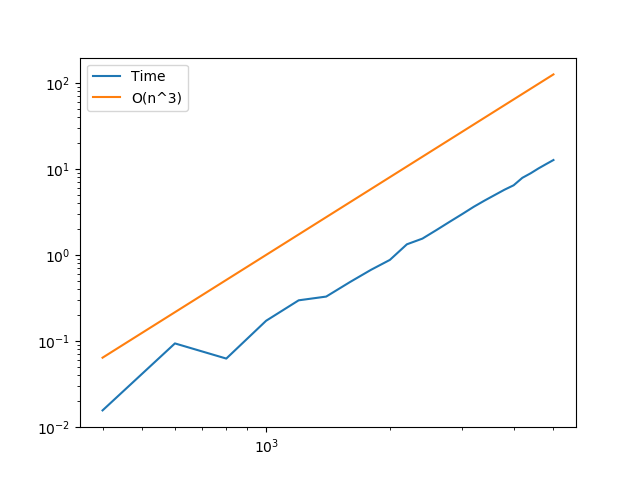
\includegraphics[width=\linewidth]{Aufgabe_1/plot_a.png}
    \caption{Rechenzeit abhängig von der Problemgröße}
    \label{fig:my_label}
\end{figure}
Wie in Abbildung 1 ersichtlich verhält sich die Rechenzeit kubisch in Relation zur Problemgröße.
Zum Testen wurde eine Zufallsmatrix mit 100 Nicht-Null-Einträgen pro Zeile (nicht exakt, da die Symmetriesierung den Wert pro
Zeile verzerrt) und einer Gesamtgröße von 5000 erstellt. Der direkte Löser wurde schließlich auf die $(200k \times 200k)$-dimensionalen Ausschnitte der oberen rechten Ecke angewandt ($2 \leq k \leq 25$). Wie man sieht erreichen wir damit schon langsam die Grenze
des akzeptabel Berechenbaren, für die volle $5000\times5000$-Matrix braucht der Algorithmus schon über 10 Sekunden.
\FloatBarrier
\subsection{CG-Verfahren}
Um die Effizienz der Problemlösung zu steigern greifen wir also nicht mehr auf den direkten Löser zurück,
sondern implementieren eine optimierte Version des CG-Verfahrens.
\begin{lstlisting}[language=Python]
def cg(A,b,x0,tol):
    xt = x0
    r0 = b - np.dot(A,xt)
    d = r0
    while(np.linalg.norm(r0) > tol):
        prod = np.dot(np.transpose(r0),r0)
        prod2 = np.dot(A,d)
        alpha = prod/np.dot(np.transpose(d),prod2)
        xt = xt + alpha*d
        r0 = r0 - alpha*prod2
        beta = np.dot(np.transpose(r0),r0)/prod
        d = r0 + beta*d
    return xt
\end{lstlisting} \label{cg}
Im Vergleich dazu Algorithmus 8.10 aus dem Numerik-Skript:
\begin{flalign*}
&1: t = 0 &\\
&2: r^{(0)} = b - Ax^{(0)} &\\
&3: d^{(0)} = r^{(0)} &\\
&4: \textbf{while}~ \norm{r^{(t)}} > \textbf{TOL}~ \text{do} &\\
&5:\quad \alpha_t = \frac{r^{(t)}*d^{(t)}}{d^{(t)}*Ad^{(t)}} &\\
&6:\quad x^{(t+1)} = x^{(t)} + \alpha_td^{(t)} &\\
&7:\quad t = t + 1 &\\
&8:\quad r^{(t)} = b - Ax^{(t)} &\\
&9:\quad \beta_{t-1} = -\frac{r^{(t)}*Ad^{(t-1)}}{d^{(t-1)}*Ad^{(t-1)}} &\\
&10:\quad d^{(t)} = r^{(t)} + \beta_{t-1}d^{(t-1)} &\\
&11: \textbf{end while}&
\end{flalign*}
Die Algorithmen ähneln sich in vielen Schritten, weisen aber durchaus einige Unterschiede auf.
Daher müssen wir noch beweisen, dass die beiden Algorithmen wirklich äquivalent sind.
Wir führen den Beweis mittels Induktion über die Anzahl der Iterationen. \\
Dabei bezeichnen wir mit * die Variablen aus unserem Algorithmus und ohne * die Variablen des Algorithmus
aus dem Skript. \\
Starten wir mit dem Induktionsanfang. \\
\begin{align*}
   &A = A^*, b = b^*, x_0 = x_0^* \\
   &r_0 = b - Ax_o = b^* - A^*x_0^* = r_0^* \\
   &d_0 = r_0 = r_0^* = d_0^* \\
   &\alpha_0 = \frac{r_0^Td_0}{d_0^TAd_0} = \frac{r_0^{*T}d_0^*}{d_0^{*T}Ad_0^*} = \frac{r_0^{*T}r_0^*}{d_0^{*T}Ad_0^*} = \alpha_0^* \\
   &x_1 = x_0 + \alpha_0d_0 = x_0^* + \alpha_0^*d_0^* = x_1^* \\
   &r_1 = b - Ax_1 = b^* - A^*x_1^* = b^* - A^*x_0^* - \alpha_0^*Ad_0^* = r_0^* - \alpha_0^*A^*d_0^* = r_1^* \\
   &\beta_0 = - \frac{r_1^TAd_0}{d_0^TAd_0} = \frac{-r_1^{*T}Ad_0^*}{d_0^{*T}Ad_0^*} = \frac{-r_1^{*T}Ar_0^*}{r_0^{*T}Ar_0^*}
\end{align*}
Unter Ausnutzung der Orthogonalität der Residuen erhalten wir: $r_1^{*T}r_0^* = 0$ und somit können wir den Bruch
folgendermaßen erweitern:
\begin{align*}
  \frac{-r_1^{*T}Ar_0^*}{r_0^{*T}Ar_0^*} = \frac{r_1^{*T}r_0^* -\alpha_0^*r_1^{*T}Ar_0^*}{\alpha_0^*r_0^{*T}Ar_0^*}
\end{align*}
Nun berechen wir
\begin{align*}
  r_1^{*T}r_1^* = r_1^{*T}(r_0^*-\alpha_0^*Ad_0^*) = r_1^{*T}r_0^* - \alpha_0^*r_1^{*T}Ar_0^*
\end{align*}
und setzen $\alpha_0^* = \frac{r_0^{*T}r_0^*}{d_0^{*T}Ad_0^*}$ ein:
\begin{align*}
  \frac{r_1^{*T}r_0^* -\alpha_0^*r_1^{*T}Ar_0^*}{\alpha_0^*r_0^{*T}Ar_0^*} = \frac{r_1^{*T}r_1^*}{\frac{r_0^{*T}r_0^*}{r_0^{*T}Ar_0^*}r_0^{*T}Ar_0^*}
  = \frac{r_1{*T}r_1^*}{r_0^{*T}r_0^*} = \beta_0^* \\
  d_1 = r_1 + \beta_0d_0 = r_1^* + \beta_0^*d_0^* = d_1^*
\end{align*}
Damit haben wir die Gleichheit der Variablen nach dem ersten Schleifendurchlauf gezeigt. \\
Sei nun nach $n$ Schleifendurchläufen die Gleichheit aller vorhergehenden Variablen vorausgesetzt: \\
\begin{align*}
  \alpha_{n-1} = \alpha_{n-1}*, x_n = x_n^*, r_n = r_n^*, \beta_{n-1} = \beta_{n-1}^*, d_n = d_n^* \\
  \alpha_n = \frac{r_n^Td_n}{d_n^TAd_n} = \frac{r_n^{*T}d_n^*}{d_n^{*T}A^*d_n^*} = \frac{r_n^{*T}(r_n^* + \beta_{n-1}^*d_{n-1}^*)}{d_n^{*T}A^*d_n^*} \\
\end{align*}
Jetzt nutzen wir die Eigenschaft: $\forall~ 0 \leq j < m: r_m^Td_j = 0$ und erhalten:
\begin{align*}
  \frac{r_n^{*T}(r_n^* + \beta_{n-1}^*d_{n-1}^*)}{d_n^{*T}A^*d_n^*} = \frac{r_n^{*T}r_n^*}{d_n^{*T}A^*d_n^*} = \alpha_n^* \\
  x_{n+1} = x_n + \alpha_nd_n = x_n^* + \alpha_n^*d_n^* = x_{n+1}^* \\
  r_{n+1} = b - Ax_{n+1} = b - A(x_n + \alpha_nd_n) = b - Ax_n - \alpha_nd_n = \\
  = r_n - \alpha_nAd_n = r_n^* - \alpha_n^*A^*d_n^* = r_{n+1}^* \\
  \beta_n = - \frac{r_{n+1}^TAd_n}{d_n^TAd_n} = \frac{r_{n+1}^{*T}r_n^* - \alpha_n^*r_{n+1}^{*T}A^*d_n^*}{d_n^{*T}A^*d_n^*}
  = \frac{r_{n+1}{*T}r_{n+1}^*}{r_n^{*T}r_n^*} = \beta_n^* \\
  d_{n+1} = r_{n+1} + \beta_nd_n = r_{n+1}^* + \beta_n^*d_n^* = d_{n+1}^*
\end{align*}
Und der Beweis ist vollständig. \\

Nun stellt sich natürlich die Frage, welcher der beiden Algorithmen zu bevorzugen ist.
Nachdem sie mathematisch äquivalent sind, bleibt nur noch die Frage nach dem Aufwand zu überprüfen.
Am aufwändigsten ist natürlich die Matrix-Vektor-Multiplikation, wovon wir in unserem Algorithmus
im Gegensatz zu jenem aus dem Skript nur eine pro Schleifendurchlauf benötigen.
Zusätzlich dazu brauchen wir 3 Vektor-Vektor-Multiplikationen und 4 Vektor-Skalar-Operationen. \\
Damit erhalten wir insgesamt $n^2+7n$ Flops pro Durchlauf. \\
Im Vergleich dazu verwendet der Algorithmus aus dem Numerik-Skript pro Iteration zwei Matrix-Vektor-Multiplikationen
und ist daher aus Effizienzgründen unterlegen, da wir damit alleine schon $2n^2$ Flops pro Durchlauf brauchen. \\

Nachdem geklärt ist, in welcher Version der Algorithmus implementiert werden soll, ist es noch essentiell sich mit der
Konvergenztheorie dahinter zu beschäftigen.
Die Theorie besagt, dass das CG-Verfahren spätentens nach $n$ Durchläufen die exakte Lösung liefert und für die Iterierten
folgende Fehlerabschätzung gilt:
\begin{align*}
  \Vbraces{x^{(t)}-A^{-1}b}_A \leq 2\left(\frac{1-1/\sqrt{\kappa}}{1+1/\sqrt{\kappa}}\right)^t\Vbraces{x^{(0)}-A^{-1}b}_A, \quad t \in \N,
\end{align*}
mit der spektralen Konditionszahl $\kappa = \text{cond}_2(A)$. \\
Also sollte das Verfahren exponentiell kovergieren ($\Landau{AB^t}$) mit Konstanten\\
$A = 2\Vbraces{x^{(0)}-A^{-1}b}_A, \quad B = \frac{1-1/\sqrt{\kappa}}{1+1/\sqrt{\kappa}}$\\
Wir haben das Verfahren mit diagonaldominanten , symmetrisch, positiv definiten Zufallsmatrizen getestet. Eine weitere
Möglichkeit wäre gewesen, eine Zufallsmatrix $A$ zu erstellen und das CG-Verfahren auf $A\cdot A^T$ anzuwenden. Allerdings ist
im letzteren Fall die Konditionszahl deutlich schlechter und teilweise erreichen wir die gewünschte Toleranz erst nach über $n$
Schritten, wo wir in der Theorie ohne Rechenfehler bereits exakt sein sollten. Also haben wir uns für erstere Methode entschieden.
Interessanterweise konvergiert der Fehler wesentlich schneller gegen 0 als die obere Schranke des theoretischen Fehlerschätzers
vermuten lassen würde und unsere vorgegebene Toleranz von $10^{-8}$ wird bereits
nach etwa $400$ Iterationen erreicht, noch weit vor dem theoretisch
(bis auf Rechenfehler) garantierten exakten Resultat nach $n = 5000$ Durchläufen.
Unsere Testwerte: \\

\begin{lstlisting}[language=Python]
n = 5000
A = zufallsmatrix(n,20)
b = np.random.rand(n)
tol = 10**(-8)
x0 = np.random.rand(n)
\end{lstlisting}

\begin{figure}
    \centering
    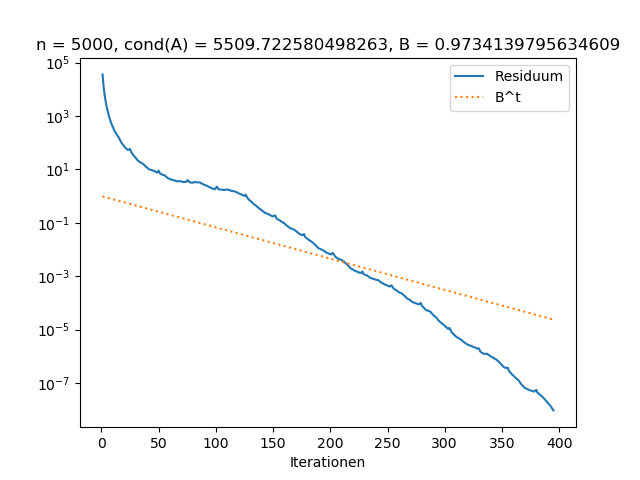
\includegraphics[width=\linewidth]{Aufgabe_1/c2.png}
    \caption{Residuum abhängig von der Anzahl an Iterationen}
    \label{fig:my_label}
\end{figure}
\FloatBarrier
\subsection{Sparse-Klasse}
Um die Effizienz weiter zu steigern, müssen wir natürlich noch die dünne Besetztheit ausnutzen.
Dies bewerkstelligen wir mit einer eigens geschrieben Klasse in Python, welche die Matrix-Vektor-Multiplikation
deutlich effizienter ausführen sollte als die Standard-Multiplikation.
Dünn besetzte Matrizen erlauben effizientere Implementierungen als voll besetzte, indem beim Speichern und Rechnen
nur Einträge die ungleich Null sind berücksichtigt werden. Eine Möglichkeit einer solchen Implementierung ist das sogenannte
\textit{compressed sparse row} Format. Anstelle aller Einträge $A_{ij}, i,j = 1,\dots,n$ einer Matrix $A \in \mathbb{R}^{n\times n}$
werden ein Vektor $v \in \mathbb{R}^{n\times n}$ aller Einträge ungleich Null, ein Vektor $J \in \mathbb{N}_0^m$ von Spaltenindizes
und ein Vektor $I \in \mathbb{N}_0^{n+1}$ von Zeigern gespeichert. Die $i$-te Zeile von $A$ ist dann gegeben durch
\begin{align*}
  A_{ij} = \begin{cases}
    v_{k(j)}, & \text{falls}~ j \in \{J_{I_i}, J_{I_i} + 1, \dots, J_{I_i + 1} - 1\} \\
    0, & \text{sonst}
  \end{cases}
\end{align*}
\begin{lstlisting}[language=Python]
class Sparse:

    def __init__(self,b,v, J = np.zeros(0), I = np.zeros(0)):
        if b:
            self.v = np.array(v)
            self.J = np.array(J)
            self.I = np.array(I)
            self.n = len(self.I)-1
        else:
            self.v, self.J, self.I = self.fromdense(v)
            self.n = len(self.I)-1

    def __matmult__(self,b):
        d = np.zeros(self.n)
        for i in range(self.n):
            x = np.array(self.J[self.I[i]:self.I[i+1]]).astype(int)
            d[i] = self.v[self.I[i]:self.I[i+1]]@b[x]
        return d


    def todense(self):
        A = np.zeros([self.n,self.n])
        for i in range(self.n):
            for j in range(self.I[i],self.I[i+1]):
                A[i][self.J[j]] = self.v[j]
        return A

    def fromdense(self,A):
        v,J = np.zeros(0), np.zeros(0)
        I = np.array([0])
        c = 0
        for i in range(np.shape(A)[0]):
            for j in range((np.shape(A))[0]):
                if A[i][j] != 0:
                    v = np.append(v,A[i][j])
                    J = np.append(J,j)
                    c += 1
            I = np.append(I,c)
        return v, J, I
\end{lstlisting}


\begin{figure}
    \centering
    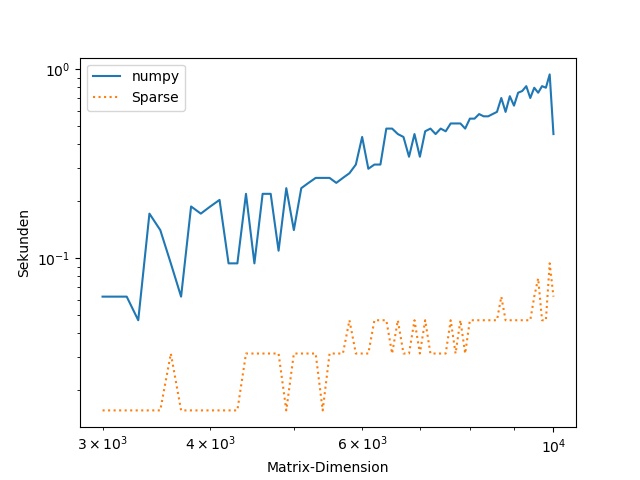
\includegraphics[width=0.8\linewidth]{Aufgabe_1/matmult_plot.png}
    \caption{Vergleich Numpy Matrixmultiplikation vs. Sparse Matrixmultiplikation}
    \label{mul}
\end{figure}
\FloatBarrier

In Abbildung \ref{mul} sehen wir, dass die Sparse-Matrix-Vektor-Multiplikation schneller ist, als die Implementierung in numpy.
Wir starten erst ab einer Matrixgröße $n=3000$, da der Messfehler bei einer kleineren Größe überwiegt und der Plot nicht aussagekräftig wäre.

\subsection{CG-Verfahren kombiniert mit Sparse-Klasse}
Jetzt können wir unsere neue Klasse noch mit der bereits vorhandenen CG-Implementierung kombinieren. \\
\begin{lstlisting}[language=Python]
def Scg(A,b,x0,tol):
    xt = x0
    r0 = b - A.__matmult__(xt)
    d = r0
    while(np.linalg.norm(r0) > tol):
        prod = np.dot(np.transpose(r0),r0)
        prod2 = A.__matmult__(d)
        alpha = prod/np.dot(np.transpose(d),prod2)
        xt = xt + alpha*d
        r0 = r0 - alpha*prod2
        beta = np.dot(np.transpose(r0),r0)/prod
        d = r0 + beta*d
    return xt
\end{lstlisting}

Bei dieser CG-Implementierung verwenden wir anstelle der Numpy-Matrix-Vektor-Multiplikation die Implementierung von der Sparse-Klasse.
Zu beachten ist, dass die Matrix A ein Objekt der Klasse Sparse sein muss, damit die Funktion durchgeführt werden kann.
Ansonsten ist die Implementierung ident zum vorherigen cg-Verfahren.
\newpage
\begin{figure}
    \centering
    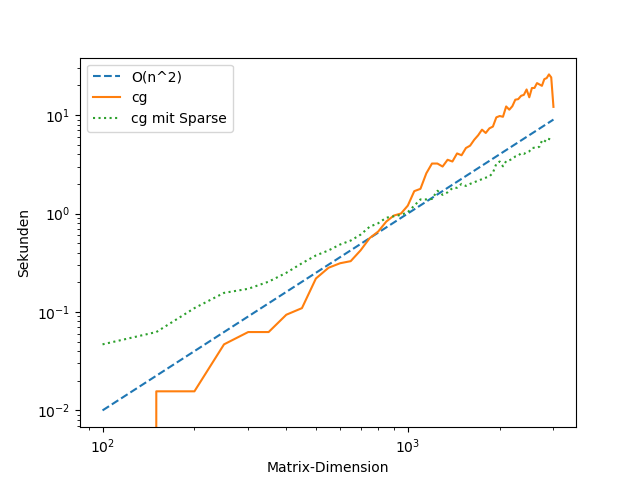
\includegraphics[width=0.9\linewidth]{Aufgabe_1/Cg_Scg.png}
    \caption{cg-Verfahren vs. cg-Verfahren mit Klasse Sparse}
    \label{scg}
\end{figure}
\FloatBarrier
Wie erhofft liefert die Kombinierung mit der Sparse-Klasse ab einer gewissen Größe noch einen zusätzlichen Effizienzschub.
Ab einer Matrixgröße von ca. 1000 ist das Scg-Verfahren effizienter als die übliche Implementierung.
Man sieht außerdem, dass beide Algorithmen eine Laufzeit von etwa $\Landau{n^2}$ (siehe Abb. \ref{scg}).

\begin{figure}
    \centering
    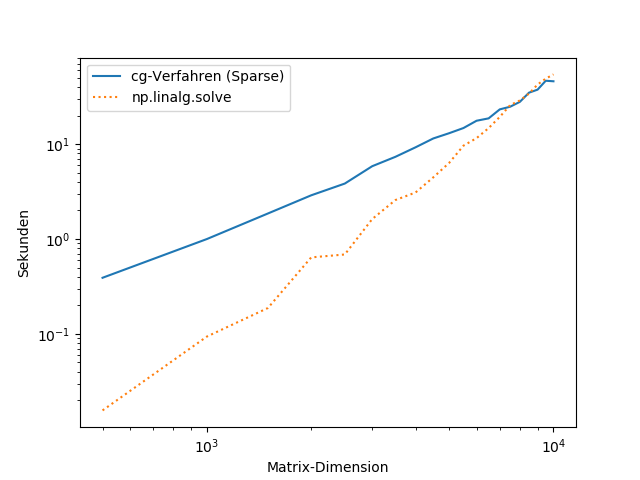
\includegraphics[width=0.8\linewidth]{Aufgabe_1/Scg_npsolve.png}
    \caption{Vergleich numpy.linalg.solve mit cg-Verfahren aus Klasse Sparse}
    \label{linalgvs}
\end{figure}
\FloatBarrier

In Abbildung \ref{linalgvs}  sieht man, dass bei kleiner Matrixgröße das Verfahren in numpy deutlich schneller als das cg-Verfahren ist, aber bei zunehmender Größe benötigt das cg-Verfahren weniger Zeit.

\subsection{Vorkonditioniertes CG-Verfahren}
Der letzte Schritt zur Effizienz-Optimierung ist nun noch die Matrix selbst noch für unsere Zwecke zu verbessern.
Die Konvergenzgeschwindigkeit des CG-Verfahrens ist durch die spektrale Konditionszahl cond($A$) der Matrix $A$ bestimmt.
Um die Konvergenzgeschwindigkeit zu erhöhen löst man das vorkonditionierte System
\begin{align*}
  D^{-1}AD^{-T} = D^{-1}b
\end{align*}
und gewinnt die Lösung $x$ dann durch $x = D^{-T}y$. Die Matrix $D$ wird dabei so gewählt, dass
\begin{itemize}
\item für beliebige Vektoren $z \in \mathbb{R}^n$ der Vektor $D^{-T}D^{-1}z$ einfach zu berechen ist und
\item $\text{cond}(D^{-1}AD^{-T}) < \text{cond}(A)$.
\end{itemize}
Implementierung des vorkonditionierten CG-Verfahrens:
\begin{lstlisting}[language=Python]
    def vcg(A,b,x0,P,tol):
        r0 = b - A.__matmult__(x0)
        P_inv = np.linalg.inv(P)
        z0 = P_inv@r0
        d = z0
        while(np.linalg.norm(r0) > tol):
            prod = np.dot(np.transpose(z0),r0)
            prod2 = A.__matmult__(d)
            alpha = np.dot(np.transpose(r0),z0)/np.dot(np.transpose(d),prod2)
            x0 = x0 + alpha*d
            r0 = r0 - alpha*prod2
            z0 = P_inv@r0
            beta = np.dot(np.transpose(z0),r0)/prod
            d = z0 + beta*d
    return x0
\end{lstlisting}

Wenn wir schließlich das vorkonditionierte CG-Verfahren mit $P = \text{diag}(A_{11},\dots,A_{nn})$ an strikt diagonaldominanten
Zufallsmatrizen mit positiven Diagonaleinträgen und an beliebigen symmetrisch, positiv definiten Zufallsmatrizen testen, sehen
wir unseren finalen Effizienzschub in diesem Projekt. \\
Wie in untenstehenden Grafik ersichtlich konnte mit der Vorkonditionierung die Anzahl der benötigten Iterationen
zur Erreichung der erwünschten Toleranz massiv gesenkt werden. Bei bereits strikt diagonaldominanten Matrizen mit positiven
Diagonaleinträgen ist die Konditionszahl
bereits relativ niedrig und somit kann die Vorkonditionierung nicht mehr so viel verbessern wie bei den normalen symmetrisch,
postiv definiten Zufallsmatrizen. Der Zeitgewinn schlägt sich bei den s.s.d. Matrizen leider nicht ganz so deutlich wieder,
aber ist dennoch vorhanden und merkbar. Bei den bereits strikt diagonaldominanten Matrizen braucht das vorkonditionierte CG-Verfahren
sogar deutlich mehr Zeit, da die Ersparnis der geringeren Anzahl an Schleifendurchläufen in diesem Fall eher minimal ist und
allerdings durch die Vorkonditionierung in jedem Iterationsschritt mehr Aufwand steckt. \\
Unsere Testwerte: Strikt diagonaldominante Matrix mit positiven Diagonaleinträgen: \\
\begin{lstlisting}[language=Python]
A = np.zeros((n,n))
row_sum = []
for i in range(n):
    non_zeros = np.random.rand(z)
    zeros = np.zeros(n-z)
    A[i] = np.concatenate((non_zeros, zeros))
    np.random.shuffle(A[i])
    row_sum.append(abs(np.sum(A[i]))+1)
A = A + A.T + np.diag(row_sum)
\end{lstlisting}
Standard s.s.d. Matrix:
\begin{lstlisting}[language=Python]
A = np.zeros((n,n))
for i in range(n):
    non_zeros = np.random.rand(z)
    zeros = np.zeros(n-z)
    A[i] = np.concatenate((non_zeros, zeros))
    np.random.shuffle(A[i])
A = A + A.T + np.diag(np.random.rand(n)*10)
\end{lstlisting}
\FloatBarrier
\begin{figure}
    \centering
    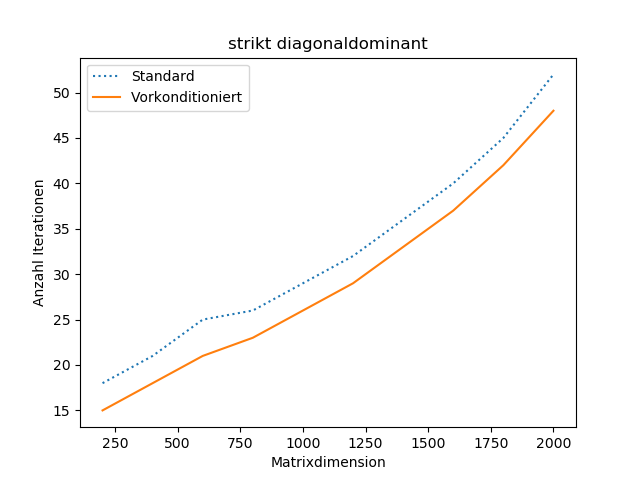
\includegraphics[width=\linewidth]{Aufgabe_1/f_strikt.png}
    \caption{strikt diagonaldominante Matrix}
\end{figure}
\begin{figure}
    \centering
    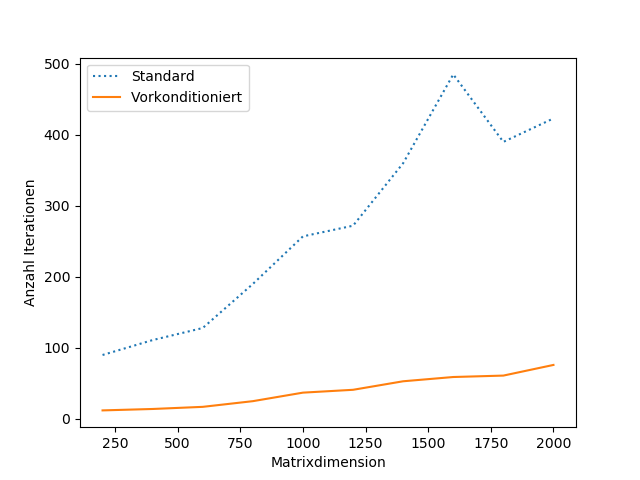
\includegraphics[width=\linewidth]{Aufgabe_1/f.png}
    \caption{s.s.d. Matrix}
\end{figure}

\begin{figure}
    \centering
    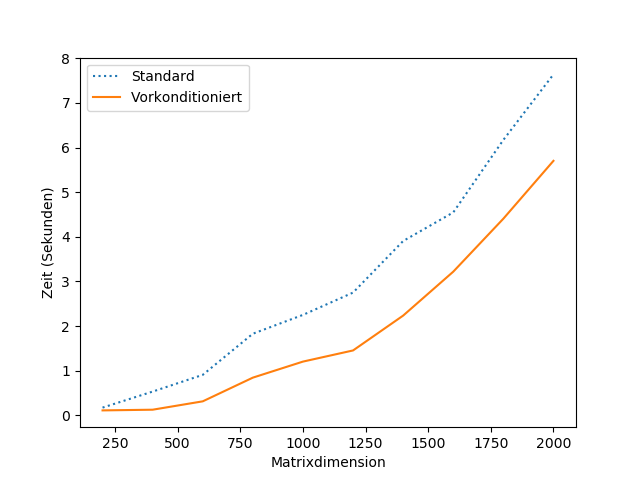
\includegraphics[width=\linewidth]{Aufgabe_1/vcg.png}
    \caption{Zeitvergleich s.s.d. Matrix}
\end{figure}

\begin{figure}
    \centering
    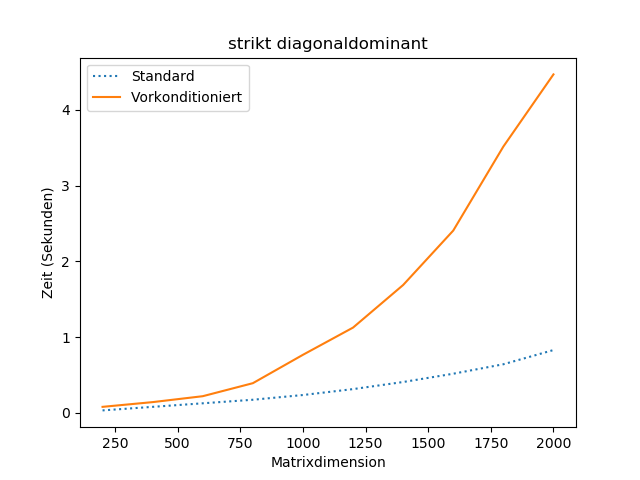
\includegraphics[width=\linewidth]{Aufgabe_1/vcg_strikt.png}
    \caption{Zeitvergleich strikt diagonaldominante Matrix}
\end{figure}

% \FloatBarrier

\section{Eigenschwingungen}
\subsection{Problembeschreibung}

Das Projekt beschäftigt sich mit den Eigenschwingeungen einer fest eingespannten Saite. Sei dazu $u(t, x)$ die vertikale Auslenkung der Saite an der Position $x \in [0, 1]$ zur Zeit $t$. $u$ wird näherungsweise durch die sogenannte Wellengleichung

\begin{align} \label{Wellengleichung}
  \frac{\partial^2 u}{\partial x^2} (t, x) =
  \frac{1}{c^2}
  \frac{\partial^2 u}{\partial t^2} (t, x)
\end{align}

für alle $x \in (0, 1)$ und $t \in \R$ beschrieben, wobei $c$ die Ausbreitungsgeschwindigkeit der Welle ist. Wenn die Saite an beiden Enden fest eingespannt ist, so gelten die Randbedingungen

\begin{align*}
  u(t, 0) = u(t, 1) = 0
\end{align*}

für alle $t \in \R$. \\

Zur Berechnung der Eigenschwingungen suchen wir nach Lösungen $u$, die in der Zeit harmonisch schwingen. Solche erfüllen folgenden Ansatz

\begin{align*}
  u(x, t) = \Re (v(x) e^{-i \omega t})
\end{align*}

mit einer festen, aber unbekannten Kreisfrequenz $\omega > 0$ und einer Funktion $v$, welche nur noch vom Ort $x$ abhängt. Durch Einsetzen erhalten wir für $v$ die sogenannte Helmholz-Gleichung

\begin{align} \label{Helmholz-Gleichung}
  -\mathbf{v}^\primeprime(x) = \kappa^2 v(x), \qquad
  x \in (0, 1),
\end{align}

mit der unbekannten Wellenzahl $\kappa := \frac{\omega}{c}$ und den Randbedingungen

\begin{align} \label{Randbedingungen}
  v(0) = v(1) = 0.
\end{align}

\subsection{Analytische Lösung}

\begin{align}
  v_\kappa(x) = C_1 \cos{(\kappa x)} + C_2 \sin{(\kappa x)}, \qquad
  x \in [0, 1],
  \label{Analytische_Lösung}
\end{align}

mit beliebigen Konstanten $C_1, C_2$, löst die Helmholz-Gleichung \eqref{Helmholz-Gleichung}. Das erkennt man durch stumpfes Einsetzen.

\begin{multline*}
  - v_\kappa^\primeprime(x)
  = - \frac{\partial^2}{\partial x^2}
    (C_1 \cos{(\kappa x)} + C_2 \sin{(\kappa x)})
  = - \frac{\partial}{\partial x}
    (- C_1 \kappa \sin{(\kappa x)} + C_2 \kappa \cos{(\kappa x)}) \\
  = - (- C_1 \kappa^2 \cos{(\kappa x)} - C_2 \kappa^2 \sin{(\kappa x)})
  = \kappa (C_1 \cos{(\kappa x)} + C_2 \sin{(\kappa x)})
  = \kappa^2 v_\kappa(x)
\end{multline*}

Wir fragen uns, für welche $\kappa > 0$, Konstanten $C_1$ und $C_2$ existieren, sodass $v_\kappa$ auch die Randbedingungen \eqref{Randbedingungen} erfüllt.

\begin{align*}
  0 \stackrel{!}{=}
  \begin{cases}
    v_\kappa(0)
    = C_1 \cos{(0)} + C_2 \sin{(0)}
    = C_1 \\
    v_\kappa(1)
    = C_1 \cos{(\kappa)} + C_2 \sin{(\kappa)}
    = C_2 \sin{(\kappa)}
  \end{cases}
\end{align*}

Nachdem $\cos{(0)} = 1$ und $\sin{(0)} = 0$ erhält man aus der oberen Gleichung $C_1 = 0$. Mit der unteren Gleichung folgt aber auch $C_2 \sin{(\kappa)} = 0$. Wenn nun auch $C_2 = 0$, dann erhielte man die triviale Lösung $v_\kappa = 0$. Für eine realistischere Modellierung, d.h. $v_\kappa \neq 0$, müsste $\sin{(\kappa)} = 0$, also $\kappa \in \pi \Z$. \\

Das sind die gesuchten $\kappa > 0$. Sei nun eines dieser $\kappa$ fest. Offensichtlich ist $C_1 = 0$ eindeutig, $C_2 \in \R$ jedoch beliebig.

\subsection{Numerische Approximation}

Häufig lassen sich solche Probleme nicht analytisch lösen, sodass auf numerische Verfahren zurückgegriffen wird, welche möglichst gute Näherungen an die exakten Lösungen berechnen sollen. Als einfachstes Mittel dienen sogenannte Differenzenverfahren. Sei dazu $x_j := jh$, $j = 0, \ldots, n$ eine Zerlegung des Intervalls $[0, 1]$ mit äquidistanter Schrittweite $h = 1/n$. Die zweite Ableitung in \eqref{Helmholz-Gleichung} wird approximiert durch den Differenzenquotienten

\begin{align} \label{Differenzenquotient}
  \mathbf{v}^\primeprime(x_j) \approx
  D_h v(x_j) :=
  \frac{1}{h^2} (v(x_{j-1}) - 2 v(x_j) + v(x_{j+1})), \qquad
  j = 1, \ldots, n-1.
\end{align}

Es sei angemerkt, dass \eqref{Differenzenquotient} tatsächlich einen Differenzenquotienten beschreibt. Um das einzusehen, verwenden wir den links- und rechts-seitigen Differenzenquotient erster Ordnung, sowie $x_{j-1} = x_j - h$, $x_{j+1} = x_j + h$. Wir erhalten $\Forall j = 1, \ldots, n-1:$

\begin{align*}
  \mathbf{v}^\primeprime(x_j)
  & = \lim_{h \to 0}
      \Frac{h}
      {
        \mathbf{v}^\prime(x_j + h) - \mathbf{v}^\prime(x_j)
      } \\
  & = \lim_{h \to 0}
      \Frac{h}
      {
        \Frac{h}
        {
          v(x_j + h) - v(x_j)
        } -
        \Frac{h}
        {
          v(x_j) - v(x_j - h)
        }
      } \\
  & = \lim_{h \to 0}
      \Frac{h^2}
      {
        v(x_j + h) - 2 v(x_j) + v(x_j - h)
      } \\
  & = \lim_{h \to 0}
      D_h v(x_j)
\end{align*}

\subsubsection{Approximationsfehler}

Für hinreichend glatte Funktionen $v$ mit einer geeigneten Konstanten $C > 0$ wird der Approximationsfehler quadratisch in $h$ klein, d.h. dass

\begin{align} \label{quadratische_Konvergenz}
  \vbraces{\mathbf{v}^\primeprime(x_j) - D_h v(x_j)} \leq C h^2.
\end{align}

Nachdem $v$ hinreichend glatt ist, gilt nach dem Satz von Taylor, dass $\Forall j = 1, \ldots, n-1:$

\begin{align*}
  v(x_j + h) & =
  \sum_{\ell = 0}^{n+2}
  \frac{h^\ell}{\ell !}
  \mathbf{v}^{(\ell)}(x_j) +
  \Landau{h^{n+3}}, \\
  v(x_j - h) & =
  \sum_{\ell = 0}^{n+2}
  \frac{(-h)^\ell}{\ell !}
  \mathbf{v}^{(\ell)}(x_j) +
  \Landau{h^{n+3}}.
\end{align*}

Man beachte, dass sich die ungeraden Summanden, der oberen Taylor-Polynome, gegenseitig aufheben. Damit erhalten wir für den Differenzenquotient $D_h v(x_j)$, $j = 1, \ldots, n-1$ eine asymptotische Entwicklung.

\begin{align*}
  D_h v(x_j)
  & = \Frac{h^2}
  {
    v(x_j - h) + v(x_j + h) - 2 v(x_j)
  } \\
  & = \Frac{h^2}
      {
        2 v(x_j) +
        h^2 \mathbf{v}^\primeprime(x_j) +
        \sum_{\substack{\ell = 4 \\ \ell \in 2 \N}}^{n+2}
        \frac{h^\ell}{\ell !}
        \mathbf{v}^{(\ell)}(x_j)
        (1 + (-1)^\ell) -
        2 v(x_j)
      } +
      \Landau{h^{n+3}} \\
  & = \mathbf{v}^\primeprime(x_j) +
      2 \sum_{\ell = 1}^\floor{\frac{n}{2}}
      \frac{h^{2 \ell}}{(2 \ell + 2)!}
      \mathbf{v}^{(2 \ell)}(x_j) +
      \Landau{h^{n+1}}
\end{align*}

Daraus folgt unmittelbar die quadratische Konvergenz \eqref{quadratische_Konvergenz}, d.h. $\Forall j = 1, \ldots, n-1:$

\begin{align*}
  D_h v(x_j) - \mathbf{v}^\primeprime(x_j) = \Landau{h^2}, \qquad
  h \to 0.
\end{align*}

\subsubsection{Eigenwertproblem}

Wir wollen nun den Differenzenquotienten $D_h v(x_j)$ verwenden, um ein Eigenwertproblem der Form $A \mathbf{v} = \lambda \mathbf{v}$ mit einer Matrix $A \in \R^{(n-1) \times (n-1)}$ zu dem Eigenvektor $\mathbf{v} := (v(x_1), \ldots, v(x_{n-1}))^T)$ und dem Eigenwert $\lambda := \kappa^2$ herzuleiten. Das soll die Helmholz-Gleichung \eqref{Helmholz-Gleichung}, mit Tupeln und Eigenwerten für die Funktionen $v_\kappa$ bzw. Vorfaktoren $\kappa$, approximieren. \\

Es wird eine Matrix $-A_n$, $n \geq 2$ gesucht, die den Differenzenquotienten $D_h v(x_j)$ auf den oberen Vektor $\mathbf{v}^{(n)}$ komponentenweise anwendet. Wir rufen in Erinnerung, dass $h = 1/n$ und definieren die naheliegende Matrix

\begin{align*}
  -A_n :=
  \frac{1}{h^2}
  \begin{pmatrix}
    -2 &  1      &        &    \\
     1 &  \ddots & \ddots &    \\
       &  \ddots & \ddots &  1 \\
       &         & 1      & -2
  \end{pmatrix}
  \in \R^{(n-1) \times (n-1)}.
\end{align*}

Wenn nun die Randbedingungen \eqref{Randbedingungen} gelten sollen, d.h. $v(x_0), v(x_n) = 0$, leistet diese Matrix $A_n$ tatsächlich das Gewünschte. Sie approximiert die linke Seite der Helmholz-Gleichung \eqref{Helmholz-Gleichung}.

\begin{align*}
  A_n \mathbf{v}^{(n)} =
  -\frac{1}{h^2}
  \begin{pmatrix}
    v(x_0) - 2 v(x_1) + v(x_2)             \\
    v(x_1) - 2 v(x_2) + v(x_3)             \\
    \vdots                                 \\
    v(x_{n-3}) - 2 v(x_{n-2}) + v(x_{n-1}) \\
    v(x_{n-2}) - 2 v(x_{n-1}) + v(x_{n-0})
  \end{pmatrix} =
  -\begin{pmatrix}
    D_h v(x_1) \\
    \vdots     \\
    D_h v(x_{n-1})
  \end{pmatrix}
  \xrightarrow{n \to \infty}
  -\mathbf{v}^\primeprime
\end{align*}

Die Matrix $A_n$ wurde in der Funktion \verb|my_numpy_matrix| implementiert. \\

\lstinputlisting
[language = Python]
{Aufgabe_2/python_code/my_numpy_matrix.py}
\vspace{10pt}

Das Eigenwertproblem wurde mit \verb|np.linalg.eig|, für beliebige $n \geq 2$, gelöst. \verb|np.linalg.eig| retourniert die Eigenwerte und Eigenvektoren nicht zwangsläufig, der größe der Eigenwerte nach, sortiert. Nachdem der Zusammenhang zwischen Eigenwert und Eigenvektor nicht verloren gehen soll, erfordert dies einigen logistischen Aufwand. Das ist aber nicht wesentlich und wird daher nicht weiter erklärt. Wir vergleichen lieber die Eigenwerte und Eigenvektoren mit den analytischen Ergebnissen. \\

In der folgenden Tabelle, sind die $3$ Eigenwerte (sollten diese bereits existieren), der Matrizen $A_2, \ldots, A_{10}$, aufgelistet. Diese Tabelle ist analog zu \eqref{Konvergenz_EW} zu verstehen. \\

\begin{tabular}{lrrrrrrrrr}
\toprule
{} &   2  &    3  &         4  &        5  &         6  &         7  &         8  &         9  &         10 \\
\midrule
1 &  8.0 &   9.0 &   9.372583 &   9.54915 &   9.646171 &   9.705051 &   9.743420 &   9.769795 &   9.788697 \\
2 &  NaN &  27.0 &  32.000000 &  34.54915 &  36.000000 &  36.897999 &  37.490332 &  37.900800 &  38.196601 \\
3 &  NaN &   NaN &  54.627417 &  65.45085 &  72.000000 &  76.192948 &  79.016521 &  81.000000 &  82.442950 \\
\bottomrule
\end{tabular}

\vspace{10pt}

Die Matrix $A_n$ besitzt also scheinbar $n-1$ paarweise verschiedene Eigenwerte $\lambda_{1, n} < \cdots < \lambda_{n-1, n}$, welche jeweils gegen $\lambda_i := (i \pi)^2$, $i \in \N$ konvergieren.

\begin{align} \label{Konvergenz_EW}
\begin{array}{ccccccccc}
\lambda_{1, 2} & \rightarrow & \lambda_{1, 3} & \rightarrow & \cdots & \rightarrow & \lambda_{1, n} & \xrightarrow{n \to \infty}   & \lambda_1 = (1 \pi)^2 \\
               &             & \lambda_{2, 3} & \rightarrow & \cdots & \rightarrow & \lambda_{2, n} & \xrightarrow{n \to \infty}   & \lambda_2 = (2 \pi)^2 \\
               &             &                &             & \ddots & \ddots      & \vdots         & \vdots                       & \vdots                \\
               &             &                &             &        &             & \lambda_{i, n} & \xrightarrow[n \to \infty]{} & \lambda_i = (i \pi)^2
\end{array}
\end{align}

Nachdem $\Bbraces{\sqrt{\lambda_i}: i \in \N_0} = \pi \N_0 \subsetneq \pi \Z$, könnte man sich nun fragen, wo die andere Hälfte der analytischen Ergebnisse steckt. Die Erklärung ist ganz unspektakulär $\lambda := (\pm \kappa)^2$. \\

Wir bezeichnen mit $\epsilon_i(n) := |\lambda_i - \lambda_{i, n}|$, $i = 1, \ldots, n-1$ den absoluten Konvergenz-Fehler des $i$-ten Eigenwertes. In der folgenden Abbildung \ref{fig:Konvergenz-Fehler_EW} wurde $\epsilon_i$ mit der Vergleich-Geraden $\id^2$, doppelt logarithmisch, geplottet. \\

\begin{figure}[H]
  \centering
  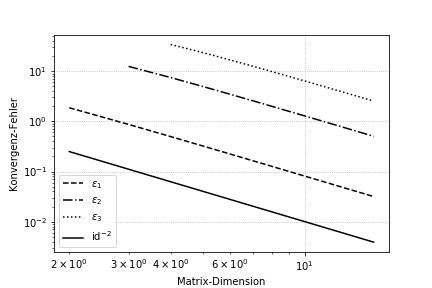
\includegraphics[width = 0.5 \textwidth]{Aufgabe_2/images/plot_eigen_value_errors(n_max = 16, i_max = 3)}
  \caption{Konvergenz-Fehler der Eigenwerte von $A_n$}
  \label{fig:Konvergenz-Fehler_EW}
\end{figure}

Allem Anschein nach, verschwindet $\epsilon_i$ quadratisch. Das korreliert mit dem Ergebnis \eqref{quadratische_Konvergenz}. Man beachte, dass der $i$-te Eigenwert erst ab einer Matrix $A_n$, $n > i$ existiert. Daher fangen die Plots von $\epsilon_i$ desto später an, je größer $i$ ist. Für größeres $i$ ist auch der intitiale Fehler größer. Obwohl dieser ebenfalls quadratisch konvergiert, werden mehr Rechenoperationen für ein genaues Ergebnis benötigt. \\

Seien $\mathbf{v}^{(1, n)}, \ldots, \mathbf{v}^{(n-1, n)}$ die Eigenvektoren (modulo Konstante), zu den Eigenwerten $\lambda_{1, n} < \cdots < \lambda_{n-1, n}$, der Matrix $A_n$. Diese sollten nun gegen die Funktionen $v_{\kappa_i}$, $\kappa_i = \sqrt{\lambda_i}$, vielleicht sogar quadratisch, konvergieren. Folgende Abbildungen sollen dies veranschaulichen.

\begin{figure}[H]
  \centering
  \subfloat[Eigenvektoren $\mathbf{v}^{(1, n)}$, $n = 2, 4, 8, 32$]{
    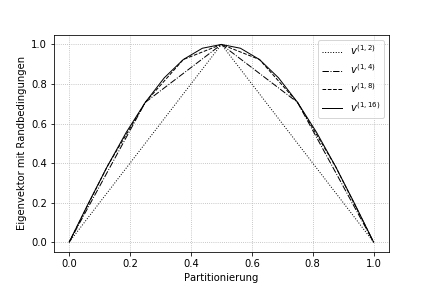
\includegraphics[width=65mm]{Aufgabe_2/images/plot_eigen_vectors/plot_eigen_vectors(n_array = [2, 4, 8, 16], i = 1).png}
  }
  \subfloat[Eigenvektoren $\mathbf{v}^{(2, n)}$, $n = 4, 8, 16, 64$]{
    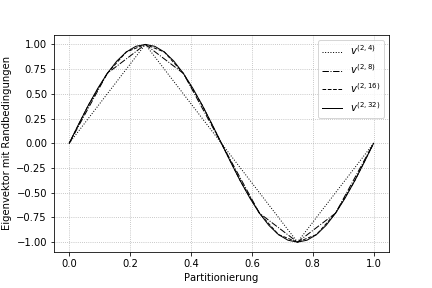
\includegraphics[width=65mm]{Aufgabe_2/images/plot_eigen_vectors/plot_eigen_vectors(n_array = [4, 8, 16, 32], i = 2).png}
  }
  \hspace{0mm}
  \subfloat[Eigenvektoren $\mathbf{v}^{(3, n)}$, $n = 8, 16, 32, 64$]{
    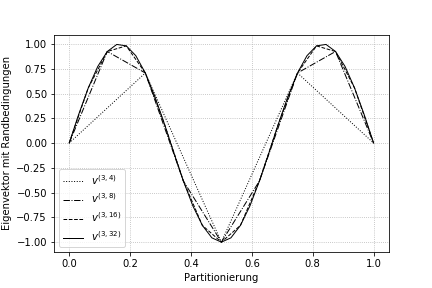
\includegraphics[width=65mm]{Aufgabe_2/images/plot_eigen_vectors/plot_eigen_vectors(n_array = [4, 8, 16, 32], i = 3).png}
  }
  \subfloat[Eigenvektoren $\mathbf{v}^{(4, n)}$, $n = 8, 16, 32, 64$]{
    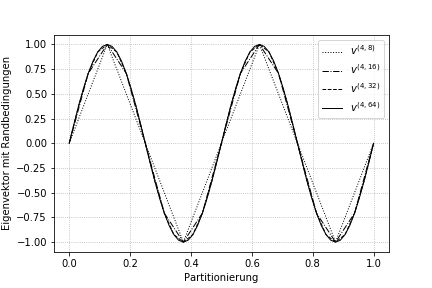
\includegraphics[width=65mm]{Aufgabe_2/images/plot_eigen_vectors/plot_eigen_vectors(n_array = [8, 16, 32, 64], i = 4).png}
  }
  \hspace{0mm}
  \caption{Eigenvektoren $\mathbf{v}^{(i, n)}$, $i = 1, \ldots, 4$ der Matrizen $A_n$}
  \label{fig:Eigenvektoren}
\end{figure}

Erstaunlicherweise, gibt es scheinbar keinen Konvergenz-Fehler, da die Eigenvektoren direkt an den Grenzfunktionen liegen. Mit anderen Worten, $\Forall n \in \N, \Forall i, j = 1, \ldots n-1:$

\begin{align*}
  \mathbf{v}^{(i, n)}_j = v_{\kappa_i}(x_j).
\end{align*}

Anschaulich, erhält man ein zu \eqref{Konvergenz_EW} analoges Schema \eqref{Konvergenz_EV}.

\begin{align} \label{Konvergenz_EV}
\begin{array}{ccccccccc}
\mathbf{v}^{(1, 2)} & \rightarrow & \mathbf{v}^{(1, 3)} & \rightarrow & \cdots & \rightarrow & \mathbf{v}^{(1, n)} & \xrightarrow{n \to \infty}   & v_{\kappa_1} \\
                &             & \mathbf{v}^{(2, 3)} & \rightarrow & \cdots & \rightarrow & \mathbf{v}^{(2, n)} & \xrightarrow{n \to \infty}   & v_{\kappa_2} \\
                &             &                 &             & \ddots & \ddots      & \vdots          & \vdots                       & \vdots       \\
                &             &                 &             &        &             & \mathbf{v}^{(i, n)} & \xrightarrow[n \to \infty]{} & v_{\kappa_i}
\end{array}
\end{align}

\subsection{Verallgemeinerte Problembeschreibung}

Die Ausbreitungsgeschwindigkeit $c$ in \eqref{Wellengleichung} hängt vom Material der Saite ab. Bisher haben wir sie als konstant angenommen, d.h. die Saite bestand aus einem Material. Sei nun für $c_0, c_1 \in \R$

\begin{align} \label{Material-Funktion}
  c(x) :=
  \begin{cases}
    c_0, x \in (0, 1/2) \\
    c_1, x \in (1/2, 1)
  \end{cases}.
\end{align}

\subsection{Verallgemeinerte Analytische Lösung}

Zuerst leiten wir eine zur Helmholz-Gleichung \eqref{Helmholz-Gleichung} ähnliche Gleichung her und geben einen \eqref{Analytische_Lösung} entsprechenden Lösungsansatz an, wenn die Lösung $v$ auf $(0, 1)$ stetig differenzierbar sein soll.
Dabei betrachten wir eine angepasste Version der Wellengleichung \eqref{Wellengleichung}.

\begin{align*}
  \frac{\partial^2 u}{\partial x^2} (t, x) =
  \frac{1}{c^2(x)}
  \frac{\partial^2 u}{\partial t^2} (t, x), \qquad
  x \in (0, 1), \qquad
  t \in \R
\end{align*}

Wir verwenden jedoch den selben Ansatz, wie Vorher. Das war $u(x, t) = \Re (v(x) e^{-i \omega t})$, mit einer festen, aber unbekannten Kreisfrequenz $\omega > 0$ und einer Funktion $v$, welche nur noch vom Ort $x$ abhängt. \\

Einsetzen und analoges Nachrechnen, gibt, mit der unbekannten Wellenzahl $\kappa(x) := \frac{\omega}{c(x)}$, die Randbedingungen \eqref{Randbedingungen} und

\begin{align*}
  -\mathbf{v}^\primeprime(x) = \kappa^2(x) v(x), \qquad
  x \in (0, 1).
\end{align*}

Um Probleme mit der Differenzierbarkeit von $\kappa$ zu vermeiden, führen wir die Abkürzungen $\kappa_0 := \frac{\omega}{c_0}$, $\kappa_1 := \frac{\omega}{c_1}$ ein, und definieren den Lösungsansatz durch Fallunterscheidung und mit (vorerst) beliebigen Konstanten $C_{01}, C_{02}, C_{11}, C_{12}$.

\begin{align*}
  v(x) :=
  \begin{cases}
    C_{01} \cos{(\kappa_0 x)} + C_{02} \sin{(\kappa_0 x)},
    & x \in (0, 1/2) \\
    C_{11} \cos{(\kappa_1 x)} + C_{12} \sin{(\kappa_1 x)},
    & x \in (1/2, 1)
  \end{cases}
\end{align*}

Durch Berücksichtigung der Randbedingungen \eqref{Randbedingungen}, erhält man (fast analog zu Vorher)

\begin{align*}
  C_{01} = 0, \qquad
  C_{11} \cos{(\kappa_1)} + C_{12} \sin{(\kappa_1)} = 0.
\end{align*}

Soll $v$ auf $1/2$ stetig fortgesetzt werden, so müssen dessen links- und rechts-seitiger Grenzwert übereinstimmen.

\begin{align*}
  C_{02} \sin(\kappa_0/2)
  = \lim_{x \to 1/2-} v(x)
  = \lim_{x \to 1/2+} v(x)
  = C_{11} \cos(\kappa_1/2) + C_{12} \sin(\kappa_1/2)
\end{align*}

Um stetige Differenzierbarkeit zu erhalten, muss auch die Ableitung

\begin{align*}
  \mathbf{v}^\prime(x) =
  \begin{cases}
    C_{02} \kappa_0 \cos(\kappa_0 x),
    & x \in (0, 1/2) \\
    - C_{11} \kappa_1 \sin(\kappa_1 x) + C_{12} \kappa_1 \cos(\kappa_1 x),
    & x \in (1/2, 1)
  \end{cases}
\end{align*}

auf $1/2$ stetig fortgesetzt werden.

\begin{align*}
  C_{02} \kappa_0 \cos(\kappa_0/2)
  = \lim_{x \to 1/2-} \mathbf{v}^\prime(x)
  = \lim_{x \to 1/2+} \mathbf{v}^\prime(x)
  = - C_{11} \kappa_1 \sin(\kappa_1/2) + C_{12} \kappa_1 \cos(\kappa_1/2)
\end{align*}

Aus den Randbedingungen und stetigen Fortsetzungen, ergibt sich also das homogene lineare Gleichungssystem $R \mathbf{C} = 0$, mit

\begin{align*}
  R :=
  \begin{pmatrix}
    \sin(\kappa_0/2)          & -\cos(\kappa_1/2)         & -\sin(\kappa_1/2) \\
    \kappa_0 \cos(\kappa_0/2) & \kappa_1 \sin(\kappa_1/2) & - \kappa_1 \cos(\kappa_1/2) \\
    0                         & \cos{\kappa_1}            & \sin{\kappa_1}
  \end{pmatrix}
  \in \R^{3 \times 3}, \qquad
  \mathbf{C} :=
  \begin{pmatrix}
    C_{02} \\
    C_{11} \\
    C_{12}
  \end{pmatrix}
  \in \R^{3 \times 1}.
\end{align*}

Sei $R \in \GL[3]{\R}$ regulär, so ist deren Kern trivial, d.h. $\ker{R} = \Bbraces{0}$, und somit auch die Lösung $\mathbf{C} = 0$. Dieser Trivialfall wurde jedoch vorhin bereits ausgeschlossen. Darum betrachten wir $\det{R} = 0$. Mit SymPy berechnet man

\begin{align} \label{Nullfunktion}
  \nonumber
  \det{R}
  & = \sin{\left(\frac{{\kappa}_{0}}{2} \right)} \cos{\left(\frac{{\kappa}_{1}}{2} \right)} {\kappa}_{1} + \sin{\left(\frac{{\kappa}_{1}}{2} \right)} \cos{\left(\frac{{\kappa}_{0}}{2} \right)} {\kappa}_{0} \\
  & = \sin{\pbraces{\frac{\omega}{2 c_0}}}
      \cos{\pbraces{\frac{\omega}{2 c_1}}}
      \frac{\omega}{c_1} +
      \sin{\pbraces{\frac{\omega}{2 c_1}}}
      \cos{\pbraces{\frac{\omega}{2 c_0}}}
      \frac{\omega}{c_0} =: f_c(\omega)
\end{align}

Für feste $c_0$, $c_1$, lässt sich das gewünschte $\omega$, als (nicht eindeutige) Nullstelle dieser Funktion $f_c$, charakterisieren.

\subsection{Verallgemeinerte Semi-Analytische Lösung}

Das Ergebnis aus \eqref{Nullfunktion} wurde, in Form von folgender Funktion, implementiert. \\

\lstinputlisting
[language = Python]
{Aufgabe_2/python_code/get_zero_function.py}
\vspace{10pt}

Nun können wir $f_c$ für fixe $c_0, c_1$ plotten lassen. Dann bekommen wir ein besseres Verständnis dafür, welchen Startwert wir wählen sollen, um die Gleichung $f_c(\omega) = 0$, mit \verb|scipy.optimize.fsolve| lösen zu lassen. \\

Für die folgenden Plots in Abbildung \ref{fig:zero_function}, wurden die arbiträren Werte $c_0 = 100$, $c_1 = 1$ gewählt. Die davon abhängige Funktion $f_c$ ist scheinbar gerade. Das liegt an \eqref{Nullfunktion}, sowie dass $\cos$ gerade und $\sin$ ungerade ist.

\begin{figure}[H]
  \centering
  \subfloat[auf dem Intervall $(-16, 16)$]{
    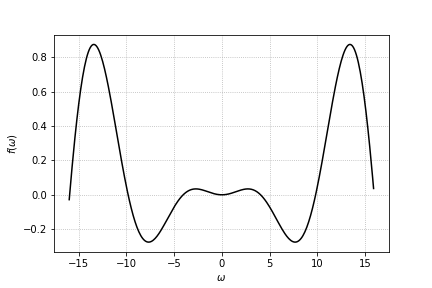
\includegraphics[width=65mm]{Aufgabe_2/images/plot_omegas/plot_omegas(c = (100, 1), interval = (-16, 16))}
  }
  \subfloat[auf dem Intervall $(0, 30)$ und herangezoomt]{
    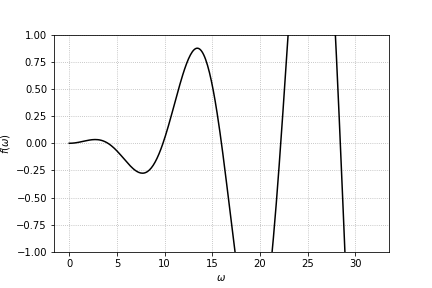
\includegraphics[width=65mm]{Aufgabe_2/images/plot_omegas/plot_omegas(c = (100, 1), interval = (0, 32), limits = (-1, 1))}
  }
  \hspace{0mm}
  \caption{Plots von $f_c$ für $c_0 = 100$, $c_1 = 1$}
  \label{fig:zero_function}
\end{figure}

Dementsprechend, können passende Startwerte $\tilde{\omega}$ für iterative Verfahren gewählt werden. Die jeweils ersten Ergebnisse $\omega$ vom, bereits erwähnten, \verb|scipy.optimize.fsolve| sind in der folgenden Tabelle. Die Quadrate $\omega^2$ dieser Ergebnisse sind Approximationen der Grenzwerte der Eigenwerte, die wir im nächsten Unterkapitel betrachten. \\

\begin{tabular}{lrrrrrr}
\toprule
{} &          1 &          2 &           3 &           4 &           5 &           6 \\
\midrule
$\tilde \omega$ &   5.000000 &  10.000000 &   15.000000 &   20.000000 &   25.000000 &   30.000000 \\
$\omega$        &   4.057425 &   9.826058 &   15.956815 &   22.170349 &   15.956815 &   28.413934 \\
$\omega^2$      &  16.462695 &  96.551423 &  254.619961 &  491.524375 &  254.619961 &  807.351663 \\
\bottomrule
\end{tabular}

\vspace{10pt}

\subsection{Verallgemeinertes Eigenwertproblem}

Wir wollen nun den Differenzenquotienten $D_h v(x_j)$ verwenden, um ein verallgemeintertes Eigenwertproblem der Form $A \mathbf{v} = \lambda B \mathbf{v}$ mit Matrizen $A, B \in \R^{(n-1) \times (n-1)}$ herzuleiten. \\

Sei abermals $x_j := jh$, $j = 0, \ldots, n$ unsere Zerlegung des Intervalls $[0, 1]$ mit äquidistanter Schrittweite $h = 1/n$. Die Matrix $-A_n$, für den Differenzenquotienten $D_h v(x_j)$, und der Vektor $\mathbf{v}^{(n)} := (v(x_1), \ldots, v(x_{n-1}))^T$, bleiben ebenfalls nach wie vor so, wie sie waren. \\

$B_n \lambda$ soll nun, analog zu Vorher, $\kappa^2$ repräsentieren. Diesmal, ist $\kappa$ jedoch als (stückweise konstante) Funktion zu verstehen. Also wird die Matrix $B_n$ deren Fallunterscheidungen übernehmen und $\lambda$ konstant bleiben. Es läuft darauf hinaus, dass \\

\begin{align*}
  B_n :=
  \begin{cases}
    \diag^{-2}
    (
      c_0, \ldots, c_0,
      c_1, \ldots, c_1,
    ), & n-1 \in 2 \N \\
    \diag^{-2}
    (
      c_0, \ldots, c_0,
      \frac{c_0 + c_1}{2},
      c_1, \ldots, c_1,
    ), & n-1 \in 2 \N + 1
  \end{cases},
  \qquad
  \lambda := \omega^2,
\end{align*}

wobei $c_0, c_1$ in $B_n \in \GL[n-1]{\R}$ jeweils $\floor{\frac{n-1}{2}}$-mal vorkommen. Dabei sei vorausgesetzt, dass $c_0, c_1 \neq 0$ und $c_0 + c_1 \neq 0$. Die Wahl von $B_n$ lässt sich wie folgt begründen. \\

Seien $\mathbf{a}, \mathbf{b}$ Vektoren mit gleich vielen Komponenten. Dann ist die Matrix-Vektor-Multiplikation $\cdot$, mit einer erzeugten Diagonalmatrix, äquivalent zur komponentenweisen Multiplikaiton $\odot$.

\begin{align} \label{Diagonalmatrizen}
  \diag(\mathbf{a}) \cdot \mathbf{b} =
  \mathbf{a} \odot \mathbf{b} =
  \mathbf{b} \odot \mathbf{a} =
  \diag(\mathbf{b}) \cdot \mathbf{a}
\end{align}

Bei dem vorherigen Eigenwertproblem wäre $B_n$ als Einheits-Matrix $I_n$ zu interpretieren. Der Eigenwert $\lambda$ konnte gleich ganz $\kappa^2$ approximieren, weil dieser Wert konstant war. Man hätte aber freilich auch mit der Skalarmatrix $(I_n c)^{-2}$ und $\omega^2$ anstelle von $\kappa^2$ arbeiten können. Da $\kappa^2$ nun aber, als Funktion, zwei unterschiedliche Werte

\begin{align*}
  \pbraces{\frac{\omega}{c_0}}^2,
  \pbraces{\frac{\omega}{c_1}}^2
\end{align*}

annehmen kann, müssen wir die obere Eigenschaft \eqref{Diagonalmatrizen} von Diagonalmatrizen ausnutzen. Damit realisieren wir die Fallunterscheidung zwischen $x_j < 1/2$ und $x_j > 1/2$. Für $x_j = 1/2$, was genau bei $n-1 \in 2 \N$ auftritt, wird gemittelt. \\

Nachdem die Inverse einer Diagonalmatrix genau die Matrix selbst mit komponentenweise Kehrwerten ist, lassen sich gleich $B_n$ und $B_n^{-1}$ leicht implementieren. Die zuständigen Funktionen besitzen die kreativen Namen \verb|my_other_numpy_matrix| bzw. \verb|my_other_numpy_matrix_inverse|. \\

\lstinputlisting
[language = Python]
{Aufgabe_2/python_code/my_other_numpy_matrices.py}
\vspace{10pt}

Das verallgemeinerte Eigenwertproblem $A_n \mathbf{v} = \lambda B_n \mathbf{v}$ werden wir zunächst auf $B_n^{-1} A_n \mathbf{v} = \lambda \mathbf{v}$ umformulieren. Dieses kann nun ebenfalls mit \verb|np.linalg.eig|, für beliebige $n \geq 2$, gelöst werden. \\

Die Matrix $B_n^{-1} A_n$ besitzt hoffentilch wieder $n-1$ paarweise verschiedene Eigenwerte $\lambda^c_{1, n} < \cdots < \lambda^c_{n-1, n}$, die jeweils konvergieren. \\

Um einen ersten Eindruck des möglichen Konvergenz-Verhaltens zu bekommen, vergleichen wir die Eigenwerte mit den oberen semi-analytischen Ergebnissen mit $c_0 = 100$, $c_1 = 1$. Es folgt eine zur oberen analoge Tabelle mit Eigenwerten. Die Ergebnisse lassen zwar zu wünschen übrig, aber immerhin pendelt sich die Größenordnung rasch ein. \\

\begin{tabular}{lrrrrr}
\toprule
{} &        2 &              3 &              4 &              5 &              6 \\
\midrule
1 &  20402.0 &      13.499662 &      21.329378 &      15.313793 &      20.048572 \\
2 &      NaN &  180004.500338 &   56813.374144 &      68.017688 &      96.940091 \\
3 &      NaN &            NaN &  344805.296478 &  250012.501563 &  102552.962302 \\
4 &      NaN &            NaN &            NaN &  750004.166956 &  422576.319931 \\
\bottomrule
\end{tabular}

\vspace{10pt}

Wir bezeichnen (optimistischerweise) mit $\epsilon_i^c(n) := |\lambda_i^c - \lambda_{i, n}^c|$, $i = 1, \ldots, n-1$ den absoluten Konvergenz-Fehler des $i$-ten Eigenwertes. $\lambda_i^c$ erhalten wir durch $\omega^2$ von \verb|scipy.optimize.fsolve|, wobei $\tilde{\omega} := \sqrt{\lambda_{i, n}^c}$ als Startwert für das iterative Verfahren gewählt wird. Theoretisch hängt $\lambda_i^c$ also noch von $n$ ab. In der folgenden Abbildung \ref{fig:Konvergenz-Fehler_EW_allgemein} wurde $\epsilon^c_i$ mit der Vergleich-Geraden $\id^2$, doppelt logarithmisch, geplottet. \\

\begin{figure}[H]
\centering
\subfloat[$c = (1, 1)$]{
  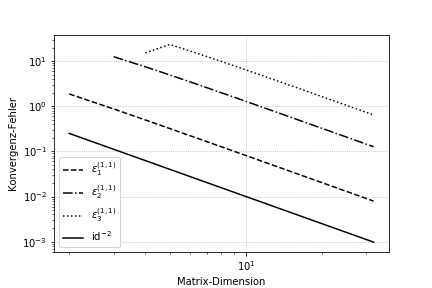
\includegraphics[width=65mm]{Aufgabe_2/images/plot_eigen_value_errors_general/plot_eigen_value_errors_general(n_max = 32, i_max = 3, c = (1, 1)).png}
  \label{subfig:Konvergenz-Fehler_EW}
}
\subfloat[$c = (1.1, 1)$]{
  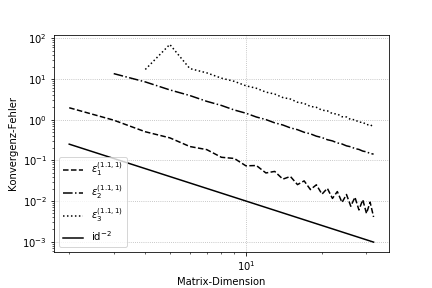
\includegraphics[width=65mm]{Aufgabe_2/images/plot_eigen_value_errors_general/plot_eigen_value_errors_general(n_max = 32, i_max = 3, c = (1.1, 1)).png}
}
\hspace{0mm}
\subfloat[$c = (2, 1)$]{
  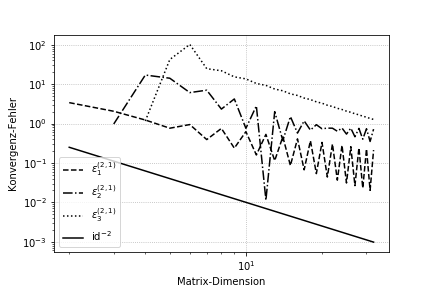
\includegraphics[width=65mm]{Aufgabe_2/images/plot_eigen_value_errors_general/plot_eigen_value_errors_general(n_max = 32, i_max = 3, c = (2, 1)).png}
  \label{Bergsteiger_a}
}
\subfloat[$c = (100, 1)$]{
  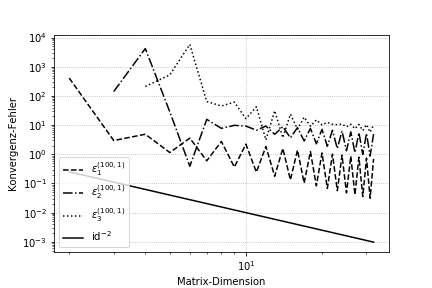
\includegraphics[width=65mm]{Aufgabe_2/images/plot_eigen_value_errors_general/plot_eigen_value_errors_general(n_max = 32, i_max = 3, c = (100, 1)).png}
  \label{Bergsteiger_b}
}
\hspace{0mm}
\caption{Konvergenz-Fehler der Eigenwerte von $B_n^{-1} A_n$, für $n = 2, \ldots, 32$ und}
\label{fig:Konvergenz-Fehler_EW_allgemein}
\end{figure}

Es macht Sinn, dass Abbildung \ref{subfig:Konvergenz-Fehler_EW} mit Abbildung \ref{fig:Konvergenz-Fehler_EW} korreliert. Diese \Quote{Bergsteiger-Konvergenz} steigt anscheinend mit dem Verhältnis $c_0/c_1$ (no pun intended). Etwas Aufschlussreicher werden \ref{Bergsteiger_a} und \ref{Bergsteiger_b}, wenn man gerade und ungerade $n$ unterscheidet. Diese Abbildung \ref{fig:Konvergenz-Fehler_EW_allgemein} bleibt übrigens unverändert, wenn man die Komponenten von $c$ vertauscht.


\begin{figure}[H]
\centering
\hspace{0mm}
\subfloat[$c = (2, 1)$, $n \in 2 \N$]{
  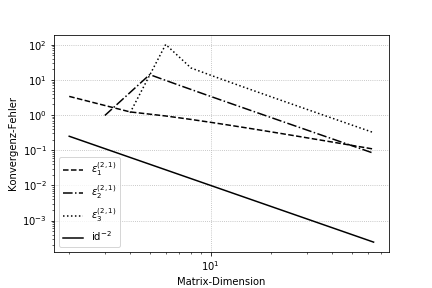
\includegraphics[width=65mm]{Aufgabe_2/images/plot_eigen_value_errors_general/plot_eigen_value_errors_general(n_max = 64, i_max = 3, c = (2, 1), parity = even).png}
}
\subfloat[$c = (100, 1)$, $n \in 2 \N$]{
  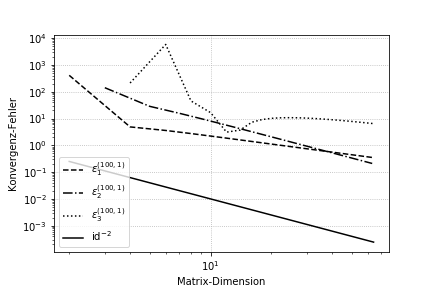
\includegraphics[width=65mm]{Aufgabe_2/images/plot_eigen_value_errors_general/plot_eigen_value_errors_general(n_max = 64, i_max = 3, c = (100, 1), parity = even).png}
  \label{gerade}
}
\hspace{0mm}
\subfloat[$c = (2, 1)$, $n \in 2 \N + 1$]{
  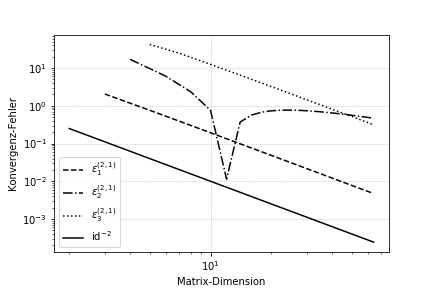
\includegraphics[width=65mm]{Aufgabe_2/images/plot_eigen_value_errors_general/plot_eigen_value_errors_general(n_max = 64, i_max = 3, c = (2, 1), parity = odd).png}
}
\subfloat[$c = (100, 1)$, $n \in 2 \N + 1$]{
  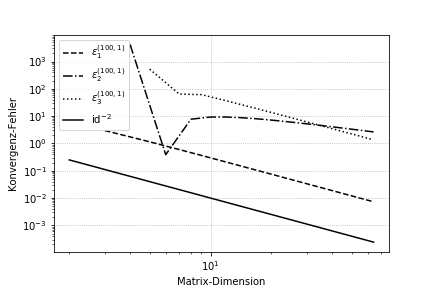
\includegraphics[width=65mm]{Aufgabe_2/images/plot_eigen_value_errors_general/plot_eigen_value_errors_general(n_max = 64, i_max = 3, c = (100, 1), parity = odd).png}
  \label{ungerade}
}
\hspace{0mm}
\caption{Konvergenz-Fehler der Eigenwerte von $B_n^{-1} A_n$, für $n = 2, \ldots, 64$ und}
\label{fig:Konvergenz-Fehler_EW_allgemein_besser}
\end{figure}

Wenn man für $c = (100, 1)$ gerade und ungerade betrachtet, so bemerkt man, dass $\epsilon_2^{(100, 1)}$ bei Abbildung \ref{gerade} konvergiert und $\epsilon_1^{(100, 1)}, \epsilon_3^{(100, 1)}$ bei Abbildung \ref{ungerade}. Dies lässt vermuten, dass im Allgemeinen die besten Approximationsstrategie ist, Teifolgen zu betrachten.

\begin{align*}
  \text{Benutze} \:
  \begin{cases}
    (\lambda_{i, n}^c)_{n \in 2 \N}     & \text{für} \: i \in 2 \N, \\
    (\lambda_{i, n}^c)_{n \in 2 \N + 1} & \text{für} \: i \in 2 \N + 1.
  \end{cases}
\end{align*}

Seien $\mathbf{v}^{(1, n), c}, \ldots, \mathbf{v}^{(n-1, n), c}$ die Eigenvektoren (modulo Konstante), zu den Eigenwerten $\lambda_{1, n}^c < \cdots < \lambda_{n-1, n}^c$, der Matrix $B_n^{-1} A_n$. Wir antizipieren ein weniger schönes Konvergenz-Verhalten, als das der Eigenvektoren der Matrizen $(A_n)_{n \in \N}$. Nichts desto trotz, wurden die Eigenvektoren $\mathbf{v}^{(i, n_i), c}$, normiert bzgl. $\norm[\infty]{\cdot}$, geplottet, wobei

\begin{align*}
  c_{\mathrm{max}} & = 4, &
  c & \in \Bbraces{(c_0, c_1): c_0, c_1 = 1, \ldots, c_{\mathrm{max}}}, \\
  i & = 1, \ldots, 2 c_{\mathrm{max}}, &
  n_i & \in \Bbraces
  {
    2^{p_{\text{min}} + p_{\text{add}}}: \:
    p_{\text{min}} = \ceil{\log_2(i+1)}, \:
    p_{\text{add}} = 0, \ldots, 3
  } =: N_i.
\end{align*}

Dabei wurden die Vektoren $\Bbraces{\mathbf{v}^{(i, n), c}: n \in N_i}$ jeweils zu einem Bild zusammengefasst. Nachdem wir dadurch auf $128$ Bilder kommen, werden wir nicht alle herzeigen. Außerdem, sieht nur ein Bruchteil davon \Quote{schön} aus. \\

\begin{figure}[H]
  \centering
  \hspace{0mm}
  \subfloat[mit $i = 2$, $n = 4, 8, 16, 32$, und $c = (1, 4)$]{
    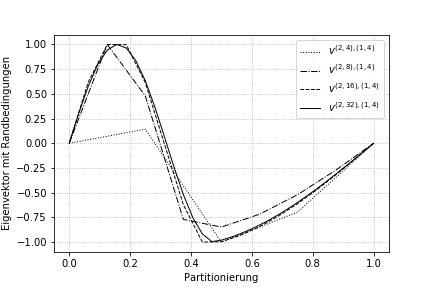
\includegraphics[width=65mm]{Aufgabe_2/images/plot_eigen_vectors_general/junk/plot_eigen_vectors_general(n_array = [4, 8, 16, 32], i = 2, c = (1, 4)).png}
  }
  \subfloat[mit $i = 6$, $n = 8, 16, 32, 64$, und $c = (1, 3)$]{
    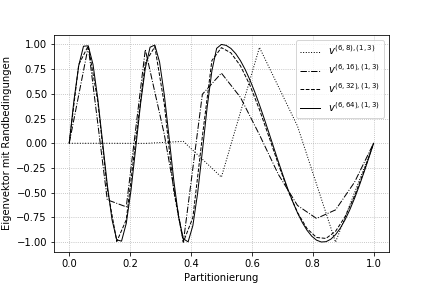
\includegraphics[width=65mm]{Aufgabe_2/images/plot_eigen_vectors_general/junk/plot_eigen_vectors_general(n_array = [8, 16, 32, 64], i = 6, c = (1, 3)).png}
  }
  \hspace{0mm}
  \subfloat[mit $i = 3$, $n = 4, 8, 16, 32$, und $c = (1, 2)$]{
    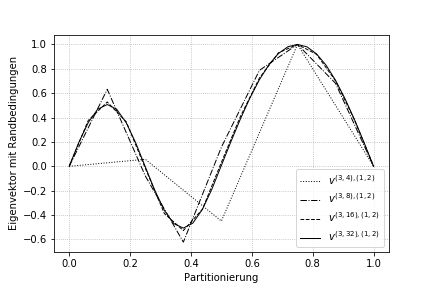
\includegraphics[width=65mm]{Aufgabe_2/images/plot_eigen_vectors_general/(1, 2), (2, 1)/plot_eigen_vectors_general(n_array = [4, 8, 16, 32], i = 3, c = (1, 2)).png}
  }
  \subfloat[mit $i = 5$, $n = 8, 16, 32, 64$, und $c = (2, 3)$]{
    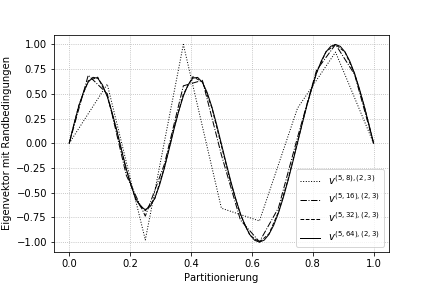
\includegraphics[width=65mm]{Aufgabe_2/images/plot_eigen_vectors_general/(2, 3), (3, 2)/plot_eigen_vectors_general(n_array = [8, 16, 32, 64], i = 5, c = (2, 3)).png}
  }
  \hspace{0mm}
  \caption{Eigenvektoren $\mathbf{v}^{(i, n), c}$ der Matrizen $B_n^{-1} A_n$}
  \label{fig:Eigenvektoren_general}
\end{figure}

Mit \Quote{schön} ist gemeint, dass die Grenzfunktionen bzgl. $n$ der Eigenvektoren $\mathbf{v}^{(i, n), c}$ seinen letzte (halbe) Schwingungs-Periode vollenden kann, bevor die nächste Ausbreitungsgeschwindigkeit übernimmt. Mit anderen Worten, die beiden Funktionshälften treffen sich an der $x$-Achse. Man fragt sich nun vielleicht, für welche Ausbreitungsgeschwindigkeiten $c$ und Eigenpaar-Nummerierung $i$ diese Grenzfunktionen \Quote{schön} aussehen. \\

Dazu bemerken wir zuerst, dass die selben Plots herauskommen, wenn $c^{(1)}, c^{(2)}$ bis auf eine Konstante übereinstimmen. Wegen der Normierung bzgl. $\norm[\infty]{\cdot}$, sieht man das durch hinschauen (auf $A \mathbf{v} = \lambda B \mathbf{v}$), also eigentilch auch bereits a priori.

\begin{align*}
  \mathbf{v}^{(i, n), c^{(1)}} = \mathbf{v}^{(i, n), c^{(2)}}, \:
  \text{für} \:
  c^{(1)} \equiv c^{(2)} \Mod \text{Konstante}.
\end{align*}

\begin{figure}[H]
  \centering
  \hspace{0mm}
  \subfloat[$c = (1, 2)$]{
    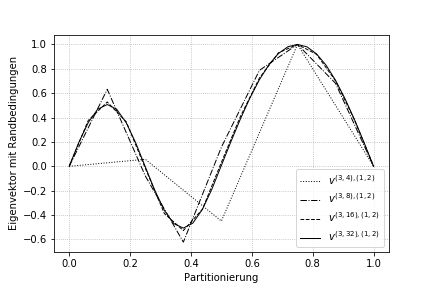
\includegraphics[width=65mm]{Aufgabe_2/images/plot_eigen_vectors_general/(1, 2), (2, 1)/plot_eigen_vectors_general(n_array = [4, 8, 16, 32], i = 3, c = (1, 2)).png}
  }
  \subfloat[$c = (2, 4)$]{
    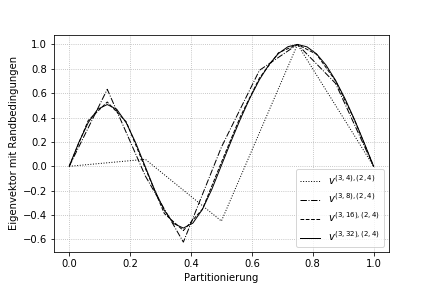
\includegraphics[width=65mm]{Aufgabe_2/images/plot_eigen_vectors_general/(1, 2), (2, 1)/plot_eigen_vectors_general(n_array = [4, 8, 16, 32], i = 3, c = (2, 4)).png}
  }
  \hspace{0mm}
  \caption{Eigenvektoren $\mathbf{v}^{(3, n), c}$ der Matrizen $B_n^{-1} A_n$, mit $n = 8, 16, 32, 64$ und}
  \label{fig:Eigenvektoren_general_Vielfache}
\end{figure}

A posteriori hingegen, bemerken wir, dass zwei Plots mit $(c_0, c_1)$ bzw. $(c_1, c_0)$ auch graphisch zusammenhängen. Die erste und zweite Hälft der Grenzfunktionen tauschen, wenn man zwischen den Plots wechselt. \\

\begin{figure}[H]
  \centering
  \hspace{0mm}
  \subfloat[$c = (1, 3)$]{
    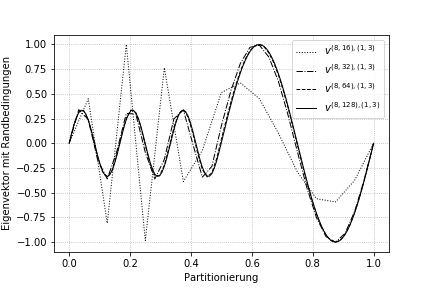
\includegraphics[width=65mm]{Aufgabe_2/images/plot_eigen_vectors_general/(1, 3), (3, 1)/plot_eigen_vectors_general(n_array = [16, 32, 64, 128], i = 8, c = (1, 3)).png}
  }
  \subfloat[$c = (3, 1)$]{
    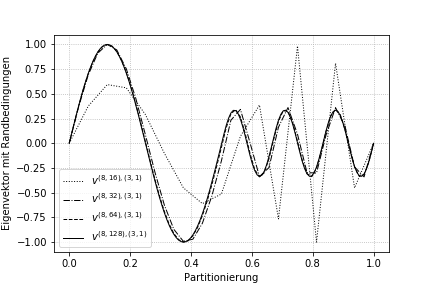
\includegraphics[width=65mm]{Aufgabe_2/images/plot_eigen_vectors_general/(1, 3), (3, 1)/plot_eigen_vectors_general(n_array = [16, 32, 64, 128], i = 8, c = (3, 1)).png}
  }
  \hspace{0mm}
  \caption{Eigenvektoren $\mathbf{v}^{(8, n), c}$ der Matrizen $B_n^{-1} A_n$, mit $n = 16, 32, 64, 128$ und}
  \label{fig:Eigenvektoren_general_vertauscht}
\end{figure}

Es sticht aber noch etwas Anderes ins Auge. Wenn man irgendeinen dieser Plots betrachtet, dann geht die Grenzfunktion genau dann durch den ausgezeichneten Punkt $(1/2, 0)$, wenn $\tilde{c_0} + \tilde{c_1} \: | \: i$, wobei $\tilde{c_0} : \tilde{c_1} = c_0 : c_1$ und $\tilde{c}$ vollständig gekürzt ist. \\

\begin{figure}[H]
  \centering
  \hspace{0mm}
  \subfloat[mit $i = 2$, $n = 4, 8, 16, 32$, und $c = (4, 4)$]{
    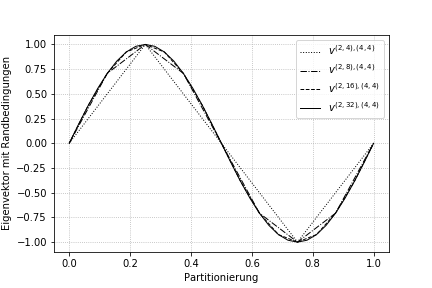
\includegraphics[width=65mm]{Aufgabe_2/images/plot_eigen_vectors_general/(1, 1)/plot_eigen_vectors_general(n_array = [4, 8, 16, 32], i = 2, c = (4, 4)).png}
  }
  \subfloat[mit $i = 4$, $n = 8, 16, 32, 64$, und $c = (1, 3)$]{
    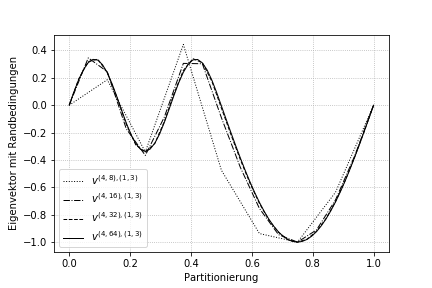
\includegraphics[width=65mm]{Aufgabe_2/images/plot_eigen_vectors_general/(1, 3), (3, 1)/plot_eigen_vectors_general(n_array = [8, 16, 32, 64], i = 4, c = (1, 3)).png}
    \label{subfig:double_trouble}
  }
  \hspace{0mm}
  \subfloat[mit $i = 8$, $n = 8, 16, 32, 64$, und $c = (1, 3)$]{
    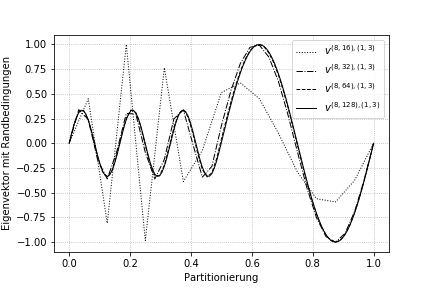
\includegraphics[width=65mm]{Aufgabe_2/images/plot_eigen_vectors_general/(1, 3), (3, 1)/plot_eigen_vectors_general(n_array = [16, 32, 64, 128], i = 8, c = (1, 3)).png}
  }
  \subfloat[mit $i = 7$, $n = 8, 16, 32, 64$, und $c = (3, 4)$]{
    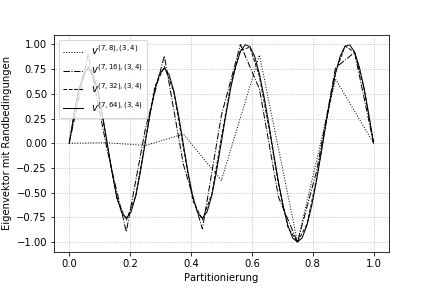
\includegraphics[width=65mm]{Aufgabe_2/images/plot_eigen_vectors_general/(3, 4), (4, 3)/plot_eigen_vectors_general(n_array = [8, 16, 32, 64], i = 7, c = (3, 4)).png}
  }
  \hspace{0mm}
  \caption{Eigenvektoren $\mathbf{v}^{(i, n), c}$ der Matrizen $B_n^{-1} A_n$}
  \label{fig:Eigenvektoren_general_nice}
\end{figure}

Das kann man heuristisch so begründen, dass die Ausbreitungsgeschwindigkeiten $c$, gemeinsam mit $i$, für die relativen Anzahlen der Schwingungsperioden verantwortlich sind; d.h, diese stehen diese im reziproken Verhältnis zu einander. Für $i = 4$, $c = (1, 3)$ aus Abbildung \ref{subfig:double_trouble} zum Beispiel, schwingt die erste Hälfte doppelt so schnell, wie die zweite. Dasselbe geschieht für $i = 8$, wobei die Grenzfunktion als Ganzes doppelt so schnell schwingt, wie bei $i = 4$. Durch dieses Zwischenspiel von $c$ und $i$, finden wir die meisten \Quote{schönen} Funktionen. \\

Was ist aber mit dem \Quote{künstlich verallgemeinerten} Fall $c = (1, 1) = \cdots = (c_{\mathrm{max}}, c_{\mathrm{max}})$, $i \in \N - 1$? Wieso sieht der so \Quote{schön} aus? Um eine Erklärung zu finden, verallgemeinern wir fröhlich weiter und betrachten die Material-Funktion $c = (c_0, \ldots, c_m) \in (\Q^+)^{m+1}$, wobei diese, analog zu \eqref{Material-Funktion}, bzgl. $1/(m+1)$ äquidistant zu verstehen ist.

\begin{align*}
  c(x) :=
  \begin{cases}
    c_0,   & x \in (0, 1/(m+1)) \\
    \vdots & \vdots \\
    c_m,   & x \in (m/(m+1), 1)
  \end{cases}
\end{align*}

Wir stellen fest, dass sich die naheliegende Verallgemeinerung der oberen Regel für diese Fälle gilt. Die Grenzfunktion geht genau dann durch die ausgezeichneten äquidistanten Punkte $\Bbraces{k/(m+1)}_{k=0}^{m+1}$, wenn $|\tilde{c}| := \tilde{c_0} + \cdots + \tilde{c_m} \: | \: i$, wobei $\tilde{c_0} : \cdots : \tilde{c_m} = c_0 : \cdots : c_m$ und $\tilde{c}$ als Ganzes vollständig gekürzt ist. \\

Tatsächlich gibt es im \Quote{künstlich verallgemeinerten} Fall mit beliebigem $i$ ein $m$, sodass für $c \in (\Q^+)^{m+1}$ gilt $|\tilde{c}| = m+1 \: | \: i$. Dieser Fall liefert übrigens, wegen der bereits angesprochenen Skalarmatrix, immer dasselbe Resultat.

\subsection{Vektor-Iteration}

Sei $\rho > 0$. Wir Verwenden die Vektor-Iteration angewendet auf das Eigenwertproblem

\begin{align} \label{geshiftetes_Eigenwertproblem}
  (A - \rho B)^{-1} B \tilde{\mathbf{v}} = \mu \tilde{\mathbf{v}}
\end{align}

mit den Matrizen $A$ und $B$ aus dem vorigen Unterkapitel. \\

Das macht man, weil die Vektor-Iteration in ihrer einfachsten Form, \verb|vector_iteration_simple|, nur den Eigenvektor mit dem betragsgrößten Eigenwert liefert. \\

\lstinputlisting
[language = Python]
{Aufgabe_2/python_code/vector_iteration_simple.py}
\vspace{10pt}

Es besteht ein Zusammenhang zwischen den Eigenpaaren $(\mu, \tilde{\mathbf{v}})$ und den Eigenpaaren $(\lambda, \mathbf{v})$ aus der vorigen Aufgabe. Für $\mu \neq 0$, ist dieser $\lambda = \rho + \frac{1}{\mu}$, weil dann

\begin{align*}
  A \mathbf{v} = \lambda B \mathbf{v}
  \Leftrightarrow
    A \mathbf{v} = \pbraces{\rho + \frac{1}{\mu}} B \mathbf{v}
  \Leftrightarrow
    B \mathbf{v} = \mu (A - \rho B) \mathbf{v}
  \Leftrightarrow
    (A - \rho B)^{-1} B \mathbf{v} = \mu \mathbf{v}.
\end{align*}

Bei der Vektor-Iteration wird der potentielle Eigenvektor $\mathbf{v}$ ständig normiert. Damit kann man wegen $A \mathbf{v} = \lambda \mathbf{v}$ sehr rasch auf den zugehörigen Eigenwert $\lambda$ kommen.

\begin{align*}
  \abraces{A \mathbf{v}, \mathbf{v}}
  = \abraces{\lambda \mathbf{v}, \mathbf{v}}
  = \lambda \norm{\mathbf{v}}^2
  = \lambda
\end{align*}

Jetzt können wir auch ein schlauereres Abbruch-Kriterium wählen. Die Vektor-Iteration soll terminieren, wenn die Änderung der Eigenwerte hinreichend klein ist. Die Implementierung, die diese Überlegungen beherzigt, folgt mit \verb|vector_iteration_unshifted|. \\

\lstinputlisting
[language = Python]
{Aufgabe_2/python_code/vector_iteration_unshifted.py}
\vspace{10pt}

Die untere Implementierung, \verb|vector_iteration_shifted|, der Vektor-Iteration des geshifteten Eigenwertproblems \eqref{geshiftetes_Eigenwertproblem}, ist ein gutes Beispiel eines sinnvollen Einsatzes der $LU$-Zerlegung. Diese ist zwar aufwändig, aber nachdem sie in jedem Iterationsschritt verwendet werden kann, zahlt sich dieser einmalige Aufwand aus. \\

\lstinputlisting
[language = Python]
{Aufgabe_2/python_code/vector_iteration_shifted.py}
\vspace{10pt}

Angenommen, wir wüssten bereits, dass all unsere Eigenwerte $\lambda_{1, n}^c < \cdots < \lambda_{n-1, n}^c \in \R^+$ reell und positiv sind. \verb|vector_iteration_simple| liefert uns den Eigenvektor mit dem betragsgrößten Eigenwert und \verb|vector_iteration_shifted| den Eigenvektor mit dem Eigenwert, der am nähesten bei $\rho$ liegt. Nun können wir mit einer binären Suche, ähnlich zum Bisektionsverfahren, alle Eigenwerte finden und ein eigenes \verb|np.linalg.eig| programmieren. \\

\lstinputlisting
[language = Python]
{Aufgabe_2/python_code/binary_search.py}
\vspace{10pt}

Das Abbruch-Kriterium ist aber anscheinend noch immer suboptimal, weil die damit berechneten Eigenwerte, sogar für \verb|tol = 1e-15|, nicht ganz denen von \verb|np.linalg.eig| entsprechen. \\

\begin{tabular}{lrrrrr}
\toprule
{} &        2 &              3 &              4 &              5 &              6 \\
\midrule
1 &  20402.0 &      13.499662 &      21.329378 &      15.313793 &      20.048572 \\
2 &      NaN &  180004.500338 &   56813.374137 &      68.003831 &      96.940090 \\
3 &      NaN &            NaN &  344805.296478 &  180595.546136 &  102552.962297 \\
4 &      NaN &            NaN &            NaN &  750004.166956 &  392219.488916 \\
\bottomrule
\end{tabular}

\vspace{10pt}

Zum Vergleich, zeigen wir nochmal die Eigenwerte via \verb|np.linalg.eig|. Betrachtet man die Eigenwerte $\lambda_{3, 5}^{(100, 1)}, \lambda_{4, 6}^{(100, 1)}$, so merkt man, dass Ungenauigkeiten beim vorletzten Eigenpaar, d.h. Eigenpaar mit betragsmäßig zweitgrößten Eigenwert, auftreten, wenn $n$ groß ist. Offensichtlich, lässt sich diese Eigenwertsuche noch optimieren, das würde aber den Rahmen dieses Projektes sprengen. \\

\begin{tabular}{lrrrrr}
\toprule
{} &        2 &              3 &              4 &              5 &              6 \\
\midrule
1 &  20402.0 &      13.499662 &      21.329378 &      15.313793 &      20.048572 \\
2 &      NaN &  180004.500338 &   56813.374144 &      68.017688 &      96.940091 \\
3 &      NaN &            NaN &  344805.296478 &  250012.501563 &  102552.962302 \\
4 &      NaN &            NaN &            NaN &  750004.166956 &  422576.319931 \\
\bottomrule
\end{tabular}

\vspace{10pt}

Zuletzt, wollen wir noch wissen, ob die Eigenwerte unserer Matrix $B_n^{-1} A_n$ tatsächlich alle positiv und reell sind. Sonst wäre der Algorithmus ja, aus mathematische Sicht, wertlos. Eine Möglichkeit bietet die explizite Darstellung von Eigenpaaren von Tridiagonalmatrizen. Wir wissen aber, dass das Gewünschte genau dann gilt, wenn $B_n^{-1} A_n$ positiv definit ist. Das können wir mit dem Hauptminoren-Kriterium locker überprüfen.

\begin{align*}
  A_n^\prime :=
  \begin{pmatrix}
     2 &  -1     &        &    \\
    -1 &  \ddots & \ddots &    \\
       &  \ddots & \ddots & -1 \\
       &         & -1     &  2
  \end{pmatrix}
\end{align*}

Zuerst berechnen wir die Determinante der Matrix $A_n^\prime$. Dazu induzieren wir $\det(A_n^\prime) = n$. Der Induktionsanfang, $n = 2, 3$, ist trivial. Für den Induktionsschritt muss man einmal nach der letzten Spalte und dann Zeile entwickeln (oder umgekehrt). \\

Nun gilt aber $A_n = \frac{1}{h^2} A_n^\prime$ und $B_n^{-1} > 0$ ist eine Diagonalmatrix mit positiven Einträgen. Weil die Determinante solcher Matrizen bloß das Produkt ihrer Komponenten ist, sind alle Hauptminoren unserer Matrizen positiv. Sie sind also tatsächlich positiv definit. Deren Produkt und Vielfaches $A_n$ ist es also auch, weil

\begin{align*}
  0 < \mathbf{x}^\ast A \mathbf{x}, \mathbf{x}^\ast B \mathbf{x}
  \Rightarrow
  0 < \mathbf{x}^\ast A \mathbf{x} \mathbf{x}^\ast B \mathbf{x} =
  \mathbf{x}^\ast A \abraces{\mathbf{x}, \mathbf{x}} B \mathbf{x} =
  \mathbf{x}^\ast A \norm{\mathbf{x}}^2 B \mathbf{x}
  \Rightarrow
  0 < \mathbf{x}^\ast AB \mathbf{x}.
\end{align*}


% \FloatBarrier
% \section{Titel}
% \subsection{Projektbeschreibung}

Sei $A$ eine symmetrische, positiv definite Matrix. Von einer \textit{Cholesky-Zerlegung} der Matrix spricht man, wenn eine untere Dreiecksmatrix
$L$ vorliegt mit $A = LL^{T}$; die Matrix $L$ und ihre Transponierte nennt man dann \textit{Choleskyfaktoren} von $A$. Ziel dieses Projekts ist die Optimierung von Algorithmen zur Berechnung einer solchen Zerlegung für schwach besetzte Matrizen (\textit{sparse matrices}).
\newline

\subsection{Lösung linearer Gleichungssysteme mit Vorwärts- und Rückwärtssubstitution}

Der Sinn dieser Zerlegung ist als Spezialfall einer LU-Zerlegung, dass sich das Problem $Ax=y$ auf die zwei Gleichungssysteme
\begin{align*}
    Lz = y \text{~~~und~~~} L^{T}x=z
\end{align*}
reduzieren lässt. Mit $L$ bzw. $L^{T}$ liegt nun eine untere bzw. obere Dreiecksmatrix vor, die wir bekannterweise mit Vorwärts- bzw. Rückwärtssubstitution effizient handhaben können.
Diese effizienten Algorithmen zur Lösung linearer Gleichungssysteme wollen wir nun speziell für den Choleskyfaktor $L$ implementieren. Da wir mit Python eine Programmiersprache nutzen, die Matrizen zeilenweise speichert, arbeiten wir auch mit dieser Art der Speicherung und nicht mit unteren Dreiecksmatrizen im Standardspaltenformat.

\lstset{language=Python}
\lstset{frame=lines}
\lstset{caption={Vorwärtssubstitution}}
\lstset{label={lst:code_direct}}
\lstset{basicstyle=\footnotesize}
\begin{lstlisting}
def vorw(L,b):
    n = len(b)

    x = np.zeros(n)

    for i in range(n):
        sum = 0
        for j in range(i):
            sum += L[i][j]*x[j]
        x[i] = (b[i]-sum)/L[i][i]
    return x
\end{lstlisting}

Die Rückwärtssubstitution bekommt in unserem Fall auch die untere Dreiecksmatrix $L$ als Input, arbeitet dann allerdings mit der Tatsache, dass mit $L^{T}$ eine obere Dreiecksmatrix vorliegt.

\lstset{language=Python}
\lstset{frame=lines}
\lstset{caption={Rückwärtssubstitution}}
\lstset{label={lst:code_direct}}
\lstset{basicstyle=\footnotesize}
\begin{lstlisting}
def rueckw(L,b):
    n = len(b)

    x = np.zeros(n)

    for i in [n-1-k for k in range(n)]:
        sum = 0
        for j in range(i,n):
            sum += L[j][i]*x[j]  ##L transponiert ist obere Dreiecksmatrix
        x[i] = (b[i]-sum)/L[i][i]

    return x
\end{lstlisting}

\subsection{Berechnung der Cholesky-Zerlegung}
\subsubsection{Zwei Varianten der Zerlegung}

Nun wollen wir für eine symmetrische, positiv definite Matrix $A$ ihren Choleskyfaktor $L$ berechnen. Hierfür stehen uns zwei Möglichkeiten zur Verfügung.

In der Vorlesung wurde ein Algorithmus in der folgenden Variante angegeben:
\begin{enumerate}
\itemsep0em
\item[] 1 \textbf{for} $k = 1,...,n$
\item[] 2 \qquad $L_{kk} = \sqrt{A_{kk} - \sum_{j=1}^{k-1} L_{kj}^2}$
\item[] 3 \qquad \textbf{for} $i = k+1,...,n$
\item[] 4 \qquad \qquad $L_{ik} = (A_{ik} - \sum_{j=1}^{k-1} L_{ij} L_{kj})/L_{kk}$.

\end{enumerate}


Diese Variante kann folgendermaßen implementiert werden, wobei die Summe $\sum_{j=1}^{k-1}L_{kj}^{2}$ aus Zeile $2$ dem Skalarprodukt der $k$-ten Zeile der bisherigen Matrix $L$ mit sich selbst entspricht:

\lstset{language=Python}
\lstset{frame=lines}
\lstset{caption={Zerlegung eintragsweise ohne Überschreiben}}
\lstset{label={lst:code_direct}}
\lstset{basicstyle=\footnotesize}
\begin{lstlisting}
def chol1(A):
    n = len(A)
    L = np.zeros((n,n))
    for k in range(n):
        L[k][k] = np.sqrt((A[k][k] - L[k]@L[k]))
        for i in range(k+1,n):
            L[i][k] = (A[i][k] - L[i]@L[k])/L[k][k]
    return L
\end{lstlisting}

Eine zweite Möglichkeit für die Berechnung der Choleskyfaktoren ist folgende:

\begin{enumerate}
\itemsep0em
\item[] 1 \textbf{for} $k = 1,...,n$
\item[] 2 \qquad $A_{kk} = \sqrt{A_{kk}}$
\item[] 3 \qquad \textbf{for} $i = k+1,...,n$
\item[] 4 \qquad \qquad $A_{ik} = A_{ik}/A_{kk}$
\item[] 5 \qquad \textbf{for} $i = k+1,...,n$
\item[] 6 \qquad \qquad \textbf{for} $j = i,...,n$
\item[] 7 \qquad \qquad \qquad $A_{ji} = A_{ji} - A_{jk} A_{ik}$.

\end{enumerate}

Dieser Algorithmus überschreibt den linken unteren Teil der Matrix $A$ direkt mit ihrem Choleskyfaktor und agiert nur auf Spalten. Das ist so zu verstehen, dass die for-Schleife in Zeile 3-4 die Division der $k$-ten Spalte (unterhalb der Hauptdiagonale) durch den Eintrag $A_{kk}$ ist. Auch die for-Schleife in Zeile 6-7 beschreibt, dass von der $i$-ten Spalte (unterhalb der Hauptdiagonale) die entsprechende $k$-te Spalte mal $A_{ik}$ abgezogen wird.


\lstset{language=Python}
\lstset{frame=lines}
\lstset{caption={Zerlegung spaltenweise mit Überschreiben}}
\lstset{label={lst:code_direct}}
\lstset{basicstyle=\footnotesize}
\begin{lstlisting}
def chol2(A):
     n = len(A)
     J = nuller(A)
     for k in range(n):
         A[k][k] = np.sqrt(A[k][k])
         A[k+1:n,k] = A[k+1:n,k]/A[k][k]
         for i in range(k+1,n):
             A[i:,i] -= A[i,k]*A[i:,k]

     for i in range(n):
         for j in range(i+1,n):
             A[i][j] = 0
     return A
\end{lstlisting}

Es bleibt noch zu zeigen, dass der zweite Algorithmus das Gleiche leistet wie der erste. Diese Äquivalenz zeigen wir mithilfe von Induktion für die Spalten $1,...,n$ (die Zeilenangaben beziehen sich dabei auf den nummerierten Code):

Die erste Spalte wird im zweiten Algorithmus nur einmal verändert. Dabei wird der Eintrag $A_{11}$ mit seiner Wurzel überschrieben und alle Einträge unter der Hauptdiagonale werden durch das neue $A_{11}$ dividiert. Die gesamte erste Spalte von $A$ entspricht also nun der ersten Spalte von $L$ aus Algorithmus 1, da in diesem die Summen für $k=1$ jeweils leer sind.

Betrachten wir nun eine beliebige Spalte $m \leq n$ und nehmen als Induktionsvoraussetzung an, dass für jedes $k < m$ die $k$-te Spalte schon der $k$-ten Spalte von $L$ aus dem ersten Algorithmus entspricht (vor Anwendung auf die $m$-te Spalte). In jeder Schleife wird also von jedem Eintrag $A_{jm}$ der $m$-ten Spalte $L_{jk}L_{mk}$ abgezogen (Zeile 7). Diese $m-1$ Subtraktionen entsprechen $-\sum_{k=1}^{m-1}L_{jk}L_{mk}$ bzw. speziell für $j=m$ der Summe $-\sum_{k=1}^{m-1}L_{mk}^{2}$ aus Zeile 4 bzw. 2 des ersten Algorithmus.

In der $m$-ten Schleife wird nun wieder das bis dahin berechnete Diagonalelement $A_{mm}^{(1)} = A_{mm}-\sum_{k=1}^{m-1}L_{mk}^{2}$ mit der Wurzel überschrieben und die jeweiligen $A_{jm}^{(1)}$ durch das neue, korrekte Diagonalelement geteilt. Nun entspricht also auch die $m$-te Spalte von $A$ der $m$-ten Spalten des Choleskyfaktors.


\subsubsection{Vergleich des Aufwands}
Beim Vergleich der Effizienz beider Varianten stellt sich heraus, dass die erste Variante schneller ist. Würden wir mit Matrizen im Standardspaltenformat arbeiten, könnten wir uns eine verbesserte Effizienz durch die zweite Variante erwarten. Da uns aber wie bereits erwähnt mit Python zeilenweise gespeicherte Matrizen vorliegen, ist der Aufwand durch den Zugriff auf gesamte Spalten sogar größer.

Daher haben wir uns entschieden, das Projekt mit der ersten Variante der Cholesky-Zerlegung weiterzuführen.

\subsection{Steigerung der Effizienz bei gegebenen Blockmatrizen}

Unseren Code möchten wir nun testen, indem wir das Gleichungssystem $Mx=b$ für beliebige rechte Seiten $b$ mittels Choleskyzerlegung lösen. Dabei sei $M \in \R^{n^{2} \times n^{2}}$, $n \in \N$ eine Blockmatrix
\begin{align*}
    M = \left(\begin{array}{cccccc}
                A & B && \boldsymbol{0} \\
                B & \ddots & \ddots & \\
                & \ddots & \ddots & B \\
                \boldsymbol{0} && B & A
           \end{array}
     \right)
\end{align*}

bestehend aus den Blöcken $A,B \in \R^{n \times n}$ mit

\begin{align*}
    A = \left( \begin{array}{cccccc}
                4 & -1 && 0 \\
                -1 & \ddots & \ddots & \\
                & \ddots & \ddots & -1 \\
                0 && -1 & 4
         \end{array}
        \right)
\mathrm{~und~}
    B = \left(\begin{array}{cccccc}
                -1 & 0 && 0 \\
                0 & \ddots & \ddots & \\
                & \ddots & \ddots & 0 \\
                0 && 0 & -1
          \end{array}
        \right).
 \end{align*}

Da $M$ strikt diagonaldominant ist, ist sie auch positiv definit. Die Symmetrie ist offensichtlich.

%Die Tests legen nahe, dass unser bisheriger Code korrekt ist.
Bei der Berechnung der Cholesky-Zerlegung der Matrix $M$ sticht ein interessantes Muster ins Auge; für ein beliebiges $n \in \N$ ist der Choleskyfaktor $L$ stets von folgender Bauart:

\begin{align*}
    L = \left(\begin{array}{cccccc}
                C &&& \boldsymbol{0} \\
                \ast & \ast && \\
                & \ddots & \ddots & \\
                \boldsymbol{0} && \ast & \ast
           \end{array}
     \right)
\end{align*}

mit einer unteren Dreiecksmatrix $C \in \R^{n \times n}$.

Das bedeutet, dass es in der ersten Spalte nur $n+1$ Einträge ungleich 0 gibt. Insbesondere hat das nur aus Nullern bestehende linke untere Dreieck eine Schenkellänge von $n^{2}-n-1$; für große $n$ ist das der Großteil der gesamten Matrix. Wir beobachten, dass dieses Dreieck aus Nullern auch in der ursprünglichen Matrix $M$ zu finden ist. Wir müssen diese Einträge also nicht mehr berechnen und können so die Effizienz des Algorithmus steigern.

In der folgenden effizienteren Variante der Cholesky-Zerlegung nutzen wir also aus, dass wir in jeder Spalte nur maximal $n$ Einträge unter der Hauptdiagonale berechnen müssen (umgesetzt in der for-Schleife Zeile 7 und 8 -- falls weniger als $n$ Einträge unter der Hauptdiagonale vorhanden sind, wollen wir natürlich nur bis zum Ende der Matrix gehen).

\lstset{language=Python}
\lstset{frame=lines}
\lstset{caption={Effiziente Cholesky-Zerlegung der Blockmatrizen}}
\lstset{label={lst:code_direct}}
\lstset{basicstyle=\footnotesize}
\begin{lstlisting}
def efficientCholBlock(n):
    A = M(n)
    L = np.zeros((n*n,n*n))
    for k in range(n*n):
        L[k][k] = np.sqrt((A[k][k] - L[k]@L[k]))
        m = min(k+n,n*n-1)
        for i in range(k+1,m+1):
             L[i][k] = (A[i][k] - L[i]@L[k])/L[k][k]
    return L
\end{lstlisting}

Wie man der folgenden Tabelle entnehmen kann, wirkt sich der Verzicht auf die Berechnung der unnötigen Einträge stark auf die Effizienz des Algorithmus aus:


\begin{table}[htb]
\centering
\caption{Vergleich des Aufwands beider Implementierungen}
\begin{tabular}{lccc}
\toprule
\textbf{n}
&\textbf{$\frac{\mathrm{\textbf{Aufwand verbesserter Algorithmus}}}{\mathrm{\textbf{Aufwand allgemeiner Algorithmus}}}$}  & \\
	        \midrule
4 & 0.895 \\
8 & 0.339 \\
16& 0.122 \\
32& 0.059 \\
64& 0.031 \\
\end{tabular}
\end{table}

Für $n=64$, also eine Blockmatrix mit ca. 16 Millionen Einträgen, reduziert sich der Aufwand demnach um fast 97 Prozent.

\subsection{Theoretische Überlegungen zu schwach besetzten Matrizen}

Die obigen Beobachtungen lassen vermuten, dass im Allgemeinen schwach besetzte Matrizen auch schwach besetzte Choleskyfaktoren besitzen. Dies gilt nicht notwendigerweise, allerdings ist es in bestimmten Fällen möglich, die Besetzungsstruktur der Matrix auszunutzen, um den Aufwand der Zerlegung zu reduzieren. Als theoretische Grundlage dazu dient folgende Überlegung:


\begin{lemma}
Sei $A$ eine symmetrische, positiv definite Matrix und die untere Dreiecksmatrix $L$ ihr Choleskyfaktor. Sei $J_i(A) := \mathrm{min}\{ j: A_{ij} \neq 0 \}$ der erste Spaltenindex einer Zeile, an dem $A$ nicht Null ist. Dann ist $L_{ij} = 0$ für $j < J_i(A)$. In $L$ bleiben also führende Nuller in Zeilen erhalten.
\end{lemma}

\begin{proof}
Es gilt $A_{ij} = \sum_{k=1}^j L_{ik} L_{kj}^T
= \sum_{k=1}^j L_{ik} L_{jk}$. Der Eintrag $A_{ij}$ kann also als kanonisches Skalarprodukt der $i$-ten und $j$-ten Zeile von $L$ interpretiert werden. $A$ ist als positiv definite Matrix insbesondere regulär; aus dem Multiplikationssatz für Determinanten folgt sofort die Regularität von $L$ und daraus die Tatsache, dass alle Diagonaleinträge von $L$ ungleich Null sind. Wir zeigen nun $L_{ij} = 0$ für alle $j < J_i(A)$.
%Für $j = 1$ gilt $0 = A_{i1} = L_{11} L_{i1}$ und aus $L_{11} \neq 0$ folgt $L_{i1} = 0.$
Ist $j < J_i(A)$ und ist die Behauptung bereits für alle $k < j$ erfüllt, so gilt
\begin{align*}
0 = A_{ij} = \sum_{k=1}^{j-1} L_{ik} L_{jk} + L_{ij} L_{jj} = 0 + L_{ij} L_{jj} = L_{ij} L_{jj}.
\end{align*}
Aus $L_{jj} \neq 0$ schließen wir $L_{ij} = 0$.
\end{proof}

\subsection{Cholesky-Zerlegung von "`Pfeil-Matrizen"'}

Gegeben seien die Matrizen $M,N \in \R^{n \times n}$ mit den Besetzungsstrukturen

\begin{align*}
    M =
\left(\begin{array}{cccccc}
                \ast & \ast & \hdots & \ast \\
                \ast & \ast && \\
                \vdots && \ddots & \\
                \ast &&& \ast
      \end{array}
\right)
\mathrm{~und~}
    N =
\left(\begin{array}{cccccc}
                \ast &&& \ast \\
                & \ddots && \vdots \\
                && \ast & \ast \\
                \ast & \hdots & \ast & \ast
      \end{array}
\right).
\end{align*}

Mithilfe unserer implementierten Zerlegung stellen wir fest, dass die Besetzungsstrukturen der jeweiligen Choleskyfaktoren unseren Überlegungen entsprechend aussehen:

\begin{align*}
    L_{M} =
\left(\begin{array}{cccccc}
                \ast &&&\boldsymbol{0} \\
                \vdots & \ddots && \\
                \vdots & \ddots & \ddots & \\
                \ast &\cdots &\cdots & \ast
      \end{array}
\right)
\mathrm{~und~}
    L_{N} =
\left(\begin{array}{cccccc}
                \ast &&& \boldsymbol{0} \\
                & \ddots && \\
                && \ast & \\
                \ast & \hdots & \ast & \ast
      \end{array}
\right).
\end{align*}

Während der Choleskyfaktor von $M$ vollbesetzt ist, ist der von $N$ von der Gestalt eines halben Pfeils und besteht nach wie vor zum Großteil aus Nullern.

Haben wir eine Matrix der Form $M$ gegeben, möchten wir also nicht ihre dünne Besetzungsstruktur verschwenden, indem wir direkt eine Cholesky-Zerlegung durchführen. Sinnvoll wäre es, die Matrix durch Permutationen auf die Form einer Matrix $N$ zu bringen und erst im Anschluss zu zerlegen.

Offensichtlich leistet die Permutationsmatrix $P =
\left(\begin{array}{cccccc}
                &&1 \\
                & \reflectbox{$\ddots$}& \\
                1  &  &
      \end{array}
\right) $ genau
$M=P^{-1}NP$.

Die Implementierung dieser Permutation mithilfe einer Matrix $P$ würde natürlich unnötigen Speicher verbrauchen, daher bemerken wir, dass die Permutation der Umnummerierung $N_{ij} = M_{n+1-i,n+1-j}$ entspricht.

\subsection{Cholesky-Zerlegung von beliebigen schwach besetzten Matrizen}

Sei $M$ eine beliebige schwach besetzte, positiv definite symmetrische Matrix. Ähnlich wie bei den Pfeilmatrizen suchen wir eine Strategie, um durch Permutationen möglichst viele der Nuller "`linksbündig"' zu machen, um schwach besetzte Choleskyfaktoren zu erhalten und so bei der Zerlegung Aufwand zu sparen.

Folgende Strategie erfüllt dieses Ziel sehr gut:

\begin{enumerate}
    \item Wir suchen die Spalte mit den meisten Nullern. Diese wird mit der ersten Spalte getauscht.
    \item Wir suchen die Spalte mit den meisten Nullern an den Stellen, an denen die neue erste Spalte auch eine Null hat. Diese wird mit der zweiten Spalte getauscht.
    \item Wir suchen die Spalte mit den meisten Nullern an den Stellen, an denen die zweite Spalte auch eine Null hat. Diese wird mit der dritten Spalte getauscht.

    $\vdots$
\end{enumerate}

Die jeweiligen Vertauschungen speichern wir als Tupel in einem Vektor ab, der als Äquivalent zur Permutationsmatrix gesehen werden kann.

\lstset{language=Python}
\lstset{frame=lines}
\lstset{caption={Permutation einer Matrix nach obigem Schema}}
\lstset{label={lst:code_direct}}
\lstset{basicstyle=\footnotesize}
\begin{lstlisting}
def sort(A):
    p=[]
    n = len(A)
    for i in range(n):
        j = i # Spalte, die spaeter an die Stelle i gesetzt wird
        max = 0
        for k in range(i,n):
            c = 0
            for l in range(0,n):
                if(i != 0):
                    if(A[l][k] == 0 and A[l][i-1] == 0):
                        c += 1
                if(i == 0):
                    if(A[l][k] == 0):
                        c += 1

            if(c > max):
                max = c
                j = k

        if(i != j):
            p += [(i,j)]
        tmp = np.copy(A[:,i])
        A[:,i] = np.copy(A[:,j])
        A[:,j] = np.copy(tmp)
        tmp2 = np.copy(A[i,:])
        A[i,:] = np.copy(A[j,:])
        A[j,:] = np.copy(tmp2)
    return A, p
\end{lstlisting}

Offenbar ist die Inverse einer Permutationsmatrix $P$ genau ihre Transponierte.\newline Wegen $x^T (P^{-1}NP) x = x^T (P^TNP) x = (Px)^T N (Px)$ bleibt die Definitheit einer Matrix $N$ unter einer solchen Transformation erhalten (weil Permutationsmatrizen regulär sind, ist $Px \neq 0$ für $x \neq 0$).
Die permutierte Matrix ist wegen $(P^TNP)^T = P^TN^TP = P^TNP$ auch wieder symmetrisch.

Haben wir nun eine permutierte Version von $M$, die uns eine günstige Berechnung der Choleskyfaktoren ermöglicht, müssen wir uns noch überlegen, wie wir erreichen, dass nur die notwendigen Einträge berechnet werden.

Die Schwierigkeit ist, dass wir nicht wie bei den Blockmatrizen einfach nur bis zu einem gewissen Index der Spalte gehen können, da die linksbündigen Nuller nur zeilenweise geordnet sind. Da unser Algorithmus die Matrix allerdings spaltenweise durchläuft, benötigen wir eine Funktion, die uns für jede Spalte die Indizes liefert, deren Einträge nicht Null sind.

\lstset{language=Python}
\lstset{frame=lines}
\lstset{caption={Output ist eine Liste $I$, die zu jeder Spalte $k$ eine Liste $I_k$ mit den Zeilenindizes der Nichtnulleinträge von $k$ enthält}}
\lstset{label={lst:code_direct}}
\lstset{basicstyle=\footnotesize}
\begin{lstlisting}
def nichtnuller(A):
    n = len(A)
    J = []
    for i in range(n):
        c = 0
        j = 0
        while(A[i][j] == 0):
            c += 1
            j += 1
        J += [c]
    I = []
    for k in range(n):
        Ik = []
        for j in range(k+1,n):
            if J[j] <= k:
                Ik += [j]
        I += [Ik]
    return I
\end{lstlisting}


Mithilfe dieser Funktion können wir also eine effiziente Variante entwickeln, eine bereits sortierte, schwach besetzte Matrix zu zerlegen:

\lstset{language=Python}
\lstset{frame=lines}
\lstset{caption={Berechnung des Choleskyfaktors unter Ausnützung führender Nuller}}
\lstset{label={lst:code_direct}}
\lstset{basicstyle=\footnotesize}
\begin{lstlisting}
def efficientChol(A):
    n = len(A)
    L = np.zeros((n,n))
    I = nichtnuller(A)
    for k in range(n):
        L[k][k] = np.sqrt((A[k][k] - L[k]@L[k]))
        for i in I[k]:
             L[i][k] = (A[i][k] - L[i]@L[k])/L[k][k]
    return L
\end{lstlisting}
Der Code entscheidet sich vom ursprünglichen lediglich durch den Kopf der for-Schleife in Zeile 7.


Wir testen nun unsere Implementierungen für schwach besetzte Matrizen. Dazu generieren wir zufällige positiv definite, symmetrische $n\times n$-Matrizen, die ungefähr $2n$ Nichtnulleinträge haben. Die folgende Tabelle zeigt die gemittelten Werte von zehn Tests; in der dritten Spalte kann man den Anteil der benötigten Zeit des naiven Algorithmus an der Zeit, die der verbesserte Algorithmus benötigt hat, ablesen.


\begin{table}[htb]
\centering
\caption{Vergleich des Aufwands der beiden Algorithmen}
\begin{tabular}{lccc}
\toprule
\textbf{n}	& \textbf{$\frac{\mathrm{\textbf{Anzahl Nuller}}}{\mathrm{\textbf{n}}}$}
&\textbf{$\frac{\mathrm{\textbf{Aufwand verbesserter Algorithmus}}}{\mathrm{\textbf{Aufwand ursprünglicher Algorithmus}}}$}  & \\
	        \midrule

4 & 1.500 & 0.728 \\
8 & 2.500 & 0.734 \\
16 & 2.000 & 0.686 \\
32 & 2.250 & 0.628 \\
64 & 2.250 & 0.512 \\
128 & 2.172 & 0.516 \\
256 & 2.258 & 0.332 \\
512 & 2.355 & 0.418 \\
1024 & 2.248 & 0.425 \\
2048 & 2.234 & 0.406 \\
4096 & 2.213 & 0.364 \\
\end{tabular}
\end{table}

Der zweite Algorithmus schneidet also wie erwartet besser ab. Wir hätten auch folgende Strategie wählen können, um die Matrix zu permutieren:

\begin{enumerate}
    \item Wir suchen die Spalte mit den meisten Nullern. Diese wird mit der ersten Spalte getauscht.
    \item Wir suchen die Spalte mit den meisten Nullern an den Stellen, an denen die neue erste Spalte auch eine Null hat. Diese wird mit der zweiten Spalte getauscht.
    \item Wir suchen die Spalte mit den meisten Nullern an den Stellen, an denen \textbf{alle vorherigen} Spalten (in unserer Variante: nur die Spalte direkt davor) auch eine Null haben. Diese wird mit der dritten Spalte getauscht.

    $\vdots$
\end{enumerate}

In den Tests zeigt sich, dass dadurch eine noch deutlichere Steigerung der Effizienz bei der Berechnung der Choleskyzerlegung möglich ist, der größere Aufwand für das Sortieren macht diese aber wieder wett. Deshalb haben wir uns für die erste Strategie entschieden.
\newline
\newline
Zuletzt möchten wir noch zusammenfassen, wie ein ganzes lineares Gleichungssystem mithilfe der dargestellten Methoden nun gelöst werden kann:

Sei $M \in \R^{n \times n}$ eine beliebige schwach besetzte symmetrisch positiv definite Matrix. Gesucht ist die Lösung des linearen Gleichungssystems $Mx=b$. Wir finden eine Permutationsmatrix $P$, sodass gilt $M = P^{-1}NP$ mit $N$ geeignet für eine günstige Cholesky-Zerlegung. Wir können das Gleichungssystem also umschreiben in
\begin{align*}
    Mx = b \text{~~} \Leftrightarrow \text{~~} P^{-1}N\underbrace{Px}_{=\colon\widetilde{x}} = b \text{~~} \Leftrightarrow \text{~~} N\widetilde{x} = \underbrace{Pb}_{=\colon\widetilde{b}}.
\end{align*}

Die Gleichung $ N\widetilde{x} = \widetilde{b}$ können wir nun wie zu Beginn besprochen mithilfe der Cholesky-Zerlegung von $N$ und anschließender Vorwärts- und Rückwärtssubstitution lösen.\footnote{Die Vorwärts- und Rückwärtssubstitution könnte in diesem Fall mit unserem Wissen über die Besetzungsstruktur der Choleskyfaktoren natürlich auch noch effizienter implementiert werden. Darauf soll allerdings in diesem Projekt nicht eingegangen werden.} Den Lösungsvektor $\widetilde{x}$ müssen wir nun lediglich wieder mit der Matrix $P^{-1}$ rückpermutieren, um unsere gesuchte Lösung $x$ zu finden.


\end{document}
